\chapter{Problem solving by uninformed and informed search}\label{chap:1}



\section{Intelligent Agent}

\lettrine[lines=3,nindent=0em,loversize=0.5]{A}{n} Agent is a structured entities composed of Sensors and Actuators, trough which it can get information on an Environment, and subsequently this can act on the Environment.




\begin{itemize}
  \item A Rational Agent act in order to obtain the best Results.

  \item The term "percept" indicate perceptive inputs.

  \item The "percept sequence" is the chronological sequence of the perception of the agent.

  \item The behaviour of an agent is described by the "Agent Function" which describes the correspondence between any specific "percept sequence" and the consequent "action".

  \item The "Agent Function" is an abstract mathematical description of the rational agent and thus can be tabulated.

  \item The "Agent Program" is the concrete implementation of the rational agent in a real system.
\end{itemize}


\subsection{Performance measure based on the rationality assumption}
The best results requested to the agent, to be best performing, need a "performance measure", which usually occur to be a distance between answer provided by the agent and the goal itself.

Performance Measure should be structured over the effect that is desirable for the agent to obtain on the ambient, instead of infer about how the agent is supposed to act.

The "rationality" of an agent is based, as Plato taught us, on these parameters:
\begin{itemize}
  \item The knowledge of the ambient;
  \item The action that the agent can take;
  \item The Performance Measure;
  \item The perceptive sequence;
\end{itemize}

In base of these knowledge the Agent must be able to choose an action that maximize the performance measure.

A second kind of action that the agent should be able to do is to Gather Information exploring the Environment, in order to boost its performance.

A third kind of action that the agent should be able to do is to Learn in base of its own perception.

\subsection{Classification of Agent}
\begin{itemize}
  \item \textbf{Simple reflex agent}
    The simplest kind of agent is the simple reflex agent. These agents select actions on the basis of the current percept, ignoring the rest of the percept history.
    it act in base of an condition–action rule stated as:
    if event-happened then start-action
  \item \textbf{Model Based reflex Agent}
  The most effective way to handle partial observability is for the agent to keep track of the part of the world it can’t see now.
  That is, the agent should maintain some sort of internal state that depends on the percept history and thereby reflects at least some of the unobserved aspects of the current state.
  \item \textbf{Goal Based Agent}
  Knowing something about the current state of the environment is not always enough to decide what to do. The GOAL agent needs some sort of goal information that describes situations that are desirable.
  Search and planning are the subfields of AI devoted to finding action sequences that achieve the agent’s goals.
  Although the goal-based agent appears less efficient, it is more flexible because the knowledge that supports its decisions is represented explicitly and can be modified.
  \item \textbf{Utility Based Agent} We have already seen that a performance measure assigns a score to any given sequence of environment states, so it can easily distinguish between more and less desirable ways of getting to the taxi’s destination. An agent’s utility function is essentially an internalization
  of the performance measure. If the internal utility function and the external performance measure are in agreement, then an agent that chooses actions to maximize its utility will be
  rational according to the external performance measure

  \item \textbf{Learning Agent}
  A learning agent can be divided into four conceptual components.
  The most important distinction is between the "Learning Element", which is responsible for making improvements, and the "Performance Element", which is responsible for selecting external actions. The performance element is what we have previously considered
  to be the entire agent: it takes in percepts and decides on actions. The learning element uses feedback from the "Critic" on how the agent is doing and determines how the performance element should be modified to do better in the future.
  The last component of the learning agent is the "problem generator". It is responsible for suggesting actions that will lead to new and informative experiences.
\end{itemize}

\begin{figure}[h!]
\centering
\subfloat[][\emph{Simple Agent}]
{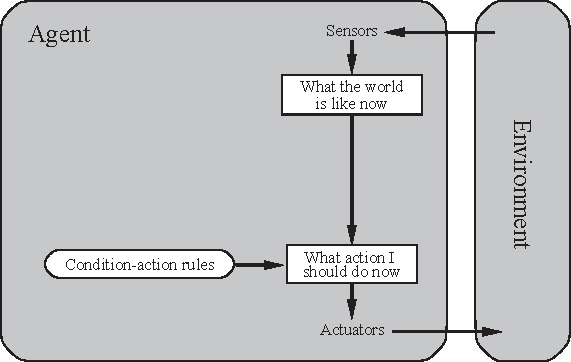
\includegraphics[width=.425\textwidth]{Simple Agent.pdf}} \qquad
\subfloat[][\emph{Goal Based Agent}]
{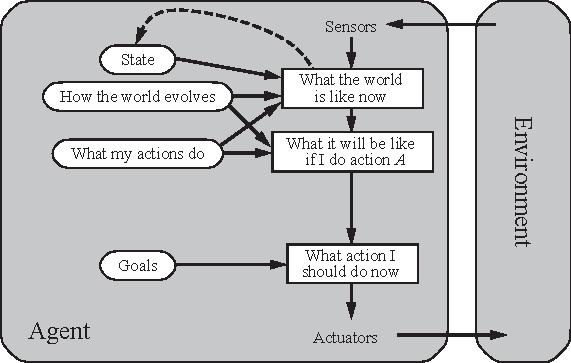
\includegraphics[width=.425\textwidth]{Goal Based.pdf}} \\
\subfloat[][\emph{Model Based Agent}]
{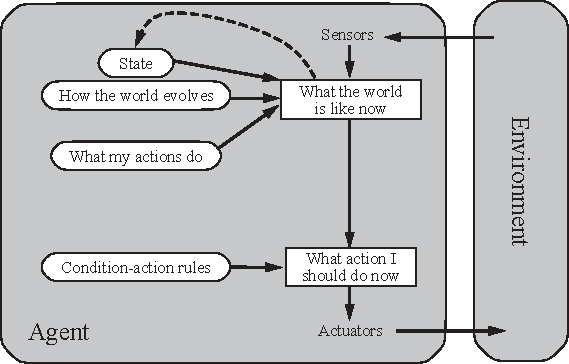
\includegraphics[width=.425\textwidth]{Model Based.pdf}} \qquad
\subfloat[][\emph{Utility Based Agent}]
{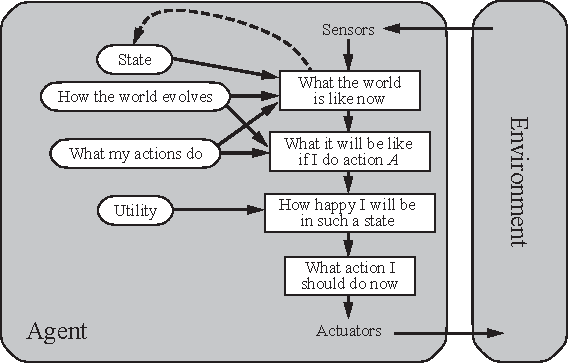
\includegraphics[width=.425\textwidth]{Utility Agent.pdf}}\\
\subfloat[][\emph{Learning Based Agent}]
{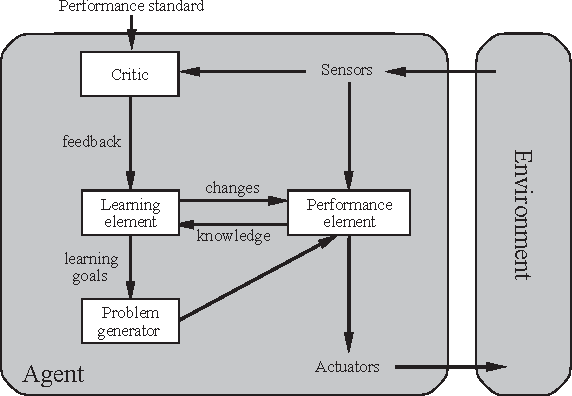
\includegraphics[width=.425\textwidth]{Learning Agent.pdf}}

\caption{Different agent models}
\label{fig:Models}
\end{figure}
%------------------------------------------------
\section{Properties of environments}

Environments come in several flavors. The principal distinctions to be made are as follows:

\begin{itemize}
  \item \textbf{Accessible vs. unaccessible}
  If an agent's sensory apparatus gives it access to the complete state of the environment, then we say that the environment is accessible to that agent. An environment is effectively accessible if the sensors detect all aspects that are relevant to the choice of action. An accessible environment is convenient because the agent need not maintain any internal state to keep track of the world.
  \item \textbf{Deterministic vs. nondeterministic}
  If the next state of the environment is completely determined by the current state and the actions selected by the agents, then we say the environment is deterministic. In principle, an agent need not worry about uncertainty in an accessible, deterministic environment. If the environment is inaccessible, however, then it may appear to be nondeterministic. This is particularly true if the environment is complex, making it hard to keep track of all the inaccessible aspects. Thus, it is often better to think of an environment as deterministic or nondeterministic from the point of view of the agent.
  \item \textbf{Episodic vs. nonepisodic}
  In an episodic environment, the agent's experience is divided into "episodes." Each episode consists of the agent perceiving and then acting. The quality of its action depends just on the episode itself, because subsequent episodes do not depend on what actions occur in previous episodes. Episodic environments are much simpler because the agent does not need to think ahead.
  \item \textbf{Static vs. dynamic}
  If the environment can change while an agent is deliberating, then we say the environment is dynamic for that agent, otherwise it is static. Static environments are easy to deal with because the agent need not keep looking at the world while it is deciding on an action,
  nor need it worry about the passage of time. If the environment does not change with the passage of time but the agent's performance score does, then we say the environment is semidynamic.
  \item \textbf{Discrete vs. continuous.}
  If there are a limited number of distinct, clearly defined percepts and actions we say that the environment is discrete. Chess is discrete—there are a fixed number of possible moves on each turn. Taxi driving is continuous—the speed and location of the taxi and the other vehicles sweep through a range of continuous values.
\end{itemize}

\section{Example problems}
\subsection{Toy problems}
\subsubsection{Missionaries and cannibals}
The missionaries and cannibals problem is usually stated as follows. Three missionaries and three cannibals are on one side of a river, along with a boat that can hold at most two people. The boat cannot cross the river by itself with no people on board. Find a way to get everyone to the other side without ever leaving a group of missionaries in one place outnumbered by the cannibals in that place (if they were, the cannibals would eat the missionaries).

There are basically two ways to solve this problem. The trivial one consists in trying manually until we get the solution (deprecated). A smarter option instead would be to reason about the possible states and legal actions (Fig.~\ref{MissionariesCannibals}). As we did in the previous sections for the vacuum-world, we start with the initial state and we build a tree diagram contemplating all possible transitions from one bank to the other. Obviously, any node that has more cannibals than missionaries on either bank is in an invalid state, and is therefore removed from further consideration. When we find a path that connects the initial states with the final one (all people in the opposite bank), then we've found one possible solution. Naturally, we expect the solutions to be infinite in number because every action can restore the environment to the previous configuration, generating a sort of loop that does not provide any help with the resolution. Nonetheless, it is possible to verify that there are 4 possible shortest solutions, each one requiring 11 boat trips.
\begin{figure}[ht]
\centering
\definecolor{River}{RGB}{51,102,204}
\resizebox{\textwidth}{!}{\newcommand{\scale}{0.36}
\begin{tikzpicture}
%\node[inner sep=0pt,outer sep=0pt] at (7.49,-1.05) {\includegraphics[width=\textwidth]{Missionaries and Cannibals Problem}};
\begin{scope}[scale=\scale,shift={(0,0)}]
\draw[line width=\scale*0.7mm,gray!75] (0.03,0.03) rectangle (5.19,3.47);
\draw[line width=\scale*0.8pt,fill=River,line join=round] plot [] coordinates {
(1.93,0)
(1.93+0.034,3.5*1/64)
(1.93+0.06,3.5*2/64)
(1.93+0.08,3.5*3/64)
(1.93+0.095,3.5*4/64)
(1.93+0.116,3.5*6/64)
(1.93+0.13,3.5*8/64)
(1.93+0.15,3.5*12/64)
(1.93+0.155,3.5*16/64)
(1.93+0.15,3.5*20/64)
(1.93+0.135,3.5*24/64)
(1.93+0.121,3.5*26/64)
(1.93+0.1,3.5*28/64)
(1.93+0.089,3.5*29/64)
(1.93+0.07,3.5*30/64)
(1.93+0.043,3.5*31/64)
(1.93,3.5*32/64)
(1.93-0.043,3.5*33/64)
(1.93-0.07,3.5*34/64)
(1.93-0.089,3.5*35/64)
(1.93-0.1,3.5*36/64)
(1.93-0.121,3.5*38/64)
(1.93-0.135,3.5*40/64)
(1.93-0.15,3.5*44/64)
(1.93-0.155,3.5*48/64)
(1.93-0.15,3.5*52/64)
(1.93-0.13,3.5*56/64)
(1.93-0.116,3.5*58/64)
(1.93-0.095,3.5*60/64)
(1.93-0.08,3.5*61/64)
(1.93-0.06,3.5*62/64)
(1.93-0.034,3.5*63/64)
(1.93,3.5)
(3.29,3.5)
(3.29-0.034,3.5*63/64)
(3.29-0.06,3.5*62/64)
(3.29-0.08,3.5*61/64)
(3.29-0.095,3.5*60/64)
(3.29-0.116,3.5*58/64)
(3.29-0.13,3.5*56/64)
(3.29-0.15,3.5*52/64)
(3.29-0.155,3.5*48/64)
(3.29-0.15,3.5*44/64)
(3.29-0.135,3.5*40/64)
(3.29-0.121,3.5*38/64)
(3.29-0.1,3.5*36/64)
(3.29-0.089,3.5*35/64)
(3.29-0.07,3.5*34/64)
(3.29-0.043,3.5*33/64)
(3.29,3.5*32/64)
(3.29+0.043,3.5*31/64)
(3.29+0.07,3.5*30/64)
(3.29+0.089,3.5*29/64)
(3.29+0.1,3.5*28/64)
(3.29+0.121,3.5*26/64)
(3.29+0.135,3.5*24/64)
(3.29+0.15,3.5*20/64)
(3.29+0.155,3.5*16/64)
(3.29+0.15,3.5*12/64)
(3.29+0.13,3.5*8/64)
(3.29+0.116,3.5*6/64)
(3.29+0.095,3.5*4/64)
(3.29+0.08,3.5*3/64)
(3.29+0.06,3.5*2/64)
(3.29+0.034,3.5*1/64)
(3.29,0)};
\draw[line width=\scale*0.7mm] (0,0) rectangle (5.22,3.5);
\draw[line width=\scale*0.7pt,line join=round,fill=white] (2.005,0.71) -- (2.535,0.71) -- (2.78,1.06) -- (1.76,1.06) -- cycle;
%\draw[line width=\scale*0.7pt,line join=round,fill=white] (3.41,1.75) -- (2.88,1.75) -- (2.635,2.12) -- (3.655,2.12) -- cycle;
\draw[line width=\scale*0.6pt,fill=black] (0.175,1.41) --++ (0:0.37) --++ (120:0.37) -- cycle;
\draw[line width=\scale*0.6pt,fill=black] (0.175+0.52,1.41-0.18) --++ (0:0.37) --++ (120:0.37) -- cycle;
\draw[line width=\scale*0.6pt,fill=black] (0.175+2*0.52,1.41-2*0.18) --++ (0:0.37) --++ (120:0.37) -- cycle;
\draw[line width=\scale*0.6pt,fill=red] (0.53,0.885) circle (0.174);
\draw[line width=\scale*0.6pt,fill=red] (0.53+0.52,0.885-0.18) circle (0.174);
\draw[line width=\scale*0.6pt,fill=red] (0.53+2*0.52,0.885-2*0.18) circle (0.174);
%\draw[line width=\scale*0.6pt,fill=black] (3.455,2.95) --++ (0:0.37) --++ (120:0.37) -- cycle;
%\draw[line width=\scale*0.6pt,fill=black] (3.455+0.52,2.95-0.18) --++ (0:0.37) --++ (120:0.37) -- cycle;
%\draw[line width=\scale*0.6pt,fill=black] (3.455+2*0.52,2.95-2*0.18) --++ (0:0.37) --++ (120:0.37) -- cycle;
%\draw[line width=\scale*0.6pt,fill=red] (3.81,2.425) circle (0.174);
%\draw[line width=\scale*0.6pt,fill=red] (3.81+0.52,2.425-0.18) circle (0.174);
%\draw[line width=\scale*0.6pt,fill=red] (3.81+2*0.52,2.425-2*0.18) circle (0.174);
\end{scope}
%%%%%%%%%%%%%%%%%%%%%%%%%%%%%%%%%%%%%%%%%%%%%%%%%%%%%
\begin{scope}[scale=\scale,shift={(6.76,0)}]
\draw[line width=\scale*0.7mm,gray!75] (0.03,0.03) rectangle (5.19,3.47);
\draw[line width=\scale*0.8pt,fill=River,line join=round] plot [] coordinates {
(1.93,0)
(1.93+0.034,3.5*1/64)
(1.93+0.06,3.5*2/64)
(1.93+0.08,3.5*3/64)
(1.93+0.095,3.5*4/64)
(1.93+0.116,3.5*6/64)
(1.93+0.13,3.5*8/64)
(1.93+0.15,3.5*12/64)
(1.93+0.155,3.5*16/64)
(1.93+0.15,3.5*20/64)
(1.93+0.135,3.5*24/64)
(1.93+0.121,3.5*26/64)
(1.93+0.1,3.5*28/64)
(1.93+0.089,3.5*29/64)
(1.93+0.07,3.5*30/64)
(1.93+0.043,3.5*31/64)
(1.93,3.5*32/64)
(1.93-0.043,3.5*33/64)
(1.93-0.07,3.5*34/64)
(1.93-0.089,3.5*35/64)
(1.93-0.1,3.5*36/64)
(1.93-0.121,3.5*38/64)
(1.93-0.135,3.5*40/64)
(1.93-0.15,3.5*44/64)
(1.93-0.155,3.5*48/64)
(1.93-0.15,3.5*52/64)
(1.93-0.13,3.5*56/64)
(1.93-0.116,3.5*58/64)
(1.93-0.095,3.5*60/64)
(1.93-0.08,3.5*61/64)
(1.93-0.06,3.5*62/64)
(1.93-0.034,3.5*63/64)
(1.93,3.5)
(3.29,3.5)
(3.29-0.034,3.5*63/64)
(3.29-0.06,3.5*62/64)
(3.29-0.08,3.5*61/64)
(3.29-0.095,3.5*60/64)
(3.29-0.116,3.5*58/64)
(3.29-0.13,3.5*56/64)
(3.29-0.15,3.5*52/64)
(3.29-0.155,3.5*48/64)
(3.29-0.15,3.5*44/64)
(3.29-0.135,3.5*40/64)
(3.29-0.121,3.5*38/64)
(3.29-0.1,3.5*36/64)
(3.29-0.089,3.5*35/64)
(3.29-0.07,3.5*34/64)
(3.29-0.043,3.5*33/64)
(3.29,3.5*32/64)
(3.29+0.043,3.5*31/64)
(3.29+0.07,3.5*30/64)
(3.29+0.089,3.5*29/64)
(3.29+0.1,3.5*28/64)
(3.29+0.121,3.5*26/64)
(3.29+0.135,3.5*24/64)
(3.29+0.15,3.5*20/64)
(3.29+0.155,3.5*16/64)
(3.29+0.15,3.5*12/64)
(3.29+0.13,3.5*8/64)
(3.29+0.116,3.5*6/64)
(3.29+0.095,3.5*4/64)
(3.29+0.08,3.5*3/64)
(3.29+0.06,3.5*2/64)
(3.29+0.034,3.5*1/64)
(3.29,0)};
\draw[line width=\scale*0.7mm] (0,0) rectangle (5.22,3.5);
\draw[line width=\scale*0.7pt,line join=round,fill=white] (3.41,1.75) -- (2.88,1.75) -- (2.635,2.12) -- (3.655,2.12) -- cycle;
\draw[line width=\scale*0.6pt,fill=black] (0.175+0.52,1.41-0.18) --++ (0:0.37) --++ (120:0.37) -- cycle;
\draw[line width=\scale*0.6pt,fill=black] (0.175+2*0.52,1.41-2*0.18) --++ (0:0.37) --++ (120:0.37) -- cycle;
\draw[line width=\scale*0.6pt,fill=red] (0.53+0.52,0.885-0.18) circle (0.174);
\draw[line width=\scale*0.6pt,fill=red] (0.53+2*0.52,0.885-2*0.18) circle (0.174);
\draw[line width=\scale*0.6pt,fill=black] (3.455,2.95) --++ (0:0.37) --++ (120:0.37) -- cycle;
\draw[line width=\scale*0.6pt,fill=red] (3.81,2.425) circle (0.174);
\end{scope}
%%%%%%%%%%%%%%%%%%%%%%%%%%%%%%%%%%%%%%%%%%%%%%%%%%%%%
\begin{scope}[scale=\scale,shift={(6.76,4.15)}]
\draw[line width=\scale*0.7mm,gray!75] (0.03,0.03) rectangle (5.19,3.47);
\draw[line width=\scale*0.8pt,fill=River,line join=round] plot [] coordinates {
(1.93,0)
(1.93+0.034,3.5*1/64)
(1.93+0.06,3.5*2/64)
(1.93+0.08,3.5*3/64)
(1.93+0.095,3.5*4/64)
(1.93+0.116,3.5*6/64)
(1.93+0.13,3.5*8/64)
(1.93+0.15,3.5*12/64)
(1.93+0.155,3.5*16/64)
(1.93+0.15,3.5*20/64)
(1.93+0.135,3.5*24/64)
(1.93+0.121,3.5*26/64)
(1.93+0.1,3.5*28/64)
(1.93+0.089,3.5*29/64)
(1.93+0.07,3.5*30/64)
(1.93+0.043,3.5*31/64)
(1.93,3.5*32/64)
(1.93-0.043,3.5*33/64)
(1.93-0.07,3.5*34/64)
(1.93-0.089,3.5*35/64)
(1.93-0.1,3.5*36/64)
(1.93-0.121,3.5*38/64)
(1.93-0.135,3.5*40/64)
(1.93-0.15,3.5*44/64)
(1.93-0.155,3.5*48/64)
(1.93-0.15,3.5*52/64)
(1.93-0.13,3.5*56/64)
(1.93-0.116,3.5*58/64)
(1.93-0.095,3.5*60/64)
(1.93-0.08,3.5*61/64)
(1.93-0.06,3.5*62/64)
(1.93-0.034,3.5*63/64)
(1.93,3.5)
(3.29,3.5)
(3.29-0.034,3.5*63/64)
(3.29-0.06,3.5*62/64)
(3.29-0.08,3.5*61/64)
(3.29-0.095,3.5*60/64)
(3.29-0.116,3.5*58/64)
(3.29-0.13,3.5*56/64)
(3.29-0.15,3.5*52/64)
(3.29-0.155,3.5*48/64)
(3.29-0.15,3.5*44/64)
(3.29-0.135,3.5*40/64)
(3.29-0.121,3.5*38/64)
(3.29-0.1,3.5*36/64)
(3.29-0.089,3.5*35/64)
(3.29-0.07,3.5*34/64)
(3.29-0.043,3.5*33/64)
(3.29,3.5*32/64)
(3.29+0.043,3.5*31/64)
(3.29+0.07,3.5*30/64)
(3.29+0.089,3.5*29/64)
(3.29+0.1,3.5*28/64)
(3.29+0.121,3.5*26/64)
(3.29+0.135,3.5*24/64)
(3.29+0.15,3.5*20/64)
(3.29+0.155,3.5*16/64)
(3.29+0.15,3.5*12/64)
(3.29+0.13,3.5*8/64)
(3.29+0.116,3.5*6/64)
(3.29+0.095,3.5*4/64)
(3.29+0.08,3.5*3/64)
(3.29+0.06,3.5*2/64)
(3.29+0.034,3.5*1/64)
(3.29,0)};
\draw[line width=\scale*0.7mm] (0,0) rectangle (5.22,3.5);
\draw[line width=\scale*0.7pt,line join=round,fill=white] (3.41,1.75) -- (2.88,1.75) -- (2.635,2.12) -- (3.655,2.12) -- cycle;
\draw[line width=\scale*0.6pt,fill=black] (0.175,1.41) --++ (0:0.37) --++ (120:0.37) -- cycle;
\draw[line width=\scale*0.6pt,fill=black] (0.175+0.52,1.41-0.18) --++ (0:0.37) --++ (120:0.37) -- cycle;
\draw[line width=\scale*0.6pt,fill=black] (0.175+2*0.52,1.41-2*0.18) --++ (0:0.37) --++ (120:0.37) -- cycle;
\draw[line width=\scale*0.6pt,fill=red] (0.53+2*0.52,0.885-2*0.18) circle (0.174);
\draw[line width=\scale*0.6pt,fill=red] (3.81,2.425) circle (0.174);
\draw[line width=\scale*0.6pt,fill=red] (3.81+0.52,2.425-0.18) circle (0.174);
\end{scope}
%%%%%%%%%%%%%%%%%%%%%%%%%%%%%%%%%%%%%%%%%%%%%%%%%%%%%
\begin{scope}[scale=\scale,shift={(6.76,-4.15)}]
\draw[line width=\scale*0.7mm,gray!75] (0.03,0.03) rectangle (5.19,3.47);
\draw[line width=\scale*0.8pt,fill=River,line join=round] plot [] coordinates {
(1.93,0)
(1.93+0.034,3.5*1/64)
(1.93+0.06,3.5*2/64)
(1.93+0.08,3.5*3/64)
(1.93+0.095,3.5*4/64)
(1.93+0.116,3.5*6/64)
(1.93+0.13,3.5*8/64)
(1.93+0.15,3.5*12/64)
(1.93+0.155,3.5*16/64)
(1.93+0.15,3.5*20/64)
(1.93+0.135,3.5*24/64)
(1.93+0.121,3.5*26/64)
(1.93+0.1,3.5*28/64)
(1.93+0.089,3.5*29/64)
(1.93+0.07,3.5*30/64)
(1.93+0.043,3.5*31/64)
(1.93,3.5*32/64)
(1.93-0.043,3.5*33/64)
(1.93-0.07,3.5*34/64)
(1.93-0.089,3.5*35/64)
(1.93-0.1,3.5*36/64)
(1.93-0.121,3.5*38/64)
(1.93-0.135,3.5*40/64)
(1.93-0.15,3.5*44/64)
(1.93-0.155,3.5*48/64)
(1.93-0.15,3.5*52/64)
(1.93-0.13,3.5*56/64)
(1.93-0.116,3.5*58/64)
(1.93-0.095,3.5*60/64)
(1.93-0.08,3.5*61/64)
(1.93-0.06,3.5*62/64)
(1.93-0.034,3.5*63/64)
(1.93,3.5)
(3.29,3.5)
(3.29-0.034,3.5*63/64)
(3.29-0.06,3.5*62/64)
(3.29-0.08,3.5*61/64)
(3.29-0.095,3.5*60/64)
(3.29-0.116,3.5*58/64)
(3.29-0.13,3.5*56/64)
(3.29-0.15,3.5*52/64)
(3.29-0.155,3.5*48/64)
(3.29-0.15,3.5*44/64)
(3.29-0.135,3.5*40/64)
(3.29-0.121,3.5*38/64)
(3.29-0.1,3.5*36/64)
(3.29-0.089,3.5*35/64)
(3.29-0.07,3.5*34/64)
(3.29-0.043,3.5*33/64)
(3.29,3.5*32/64)
(3.29+0.043,3.5*31/64)
(3.29+0.07,3.5*30/64)
(3.29+0.089,3.5*29/64)
(3.29+0.1,3.5*28/64)
(3.29+0.121,3.5*26/64)
(3.29+0.135,3.5*24/64)
(3.29+0.15,3.5*20/64)
(3.29+0.155,3.5*16/64)
(3.29+0.15,3.5*12/64)
(3.29+0.13,3.5*8/64)
(3.29+0.116,3.5*6/64)
(3.29+0.095,3.5*4/64)
(3.29+0.08,3.5*3/64)
(3.29+0.06,3.5*2/64)
(3.29+0.034,3.5*1/64)
(3.29,0)};
\draw[line width=\scale*0.7mm] (0,0) rectangle (5.22,3.5);
\draw[line width=\scale*0.7pt,line join=round,fill=white] (3.41,1.75) -- (2.88,1.75) -- (2.635,2.12) -- (3.655,2.12) -- cycle;
\draw[line width=\scale*0.6pt,fill=black] (0.175,1.41) --++ (0:0.37) --++ (120:0.37) -- cycle;
\draw[line width=\scale*0.6pt,fill=black] (0.175+0.52,1.41-0.18) --++ (0:0.37) --++ (120:0.37) -- cycle;
\draw[line width=\scale*0.6pt,fill=black] (0.175+2*0.52,1.41-2*0.18) --++ (0:0.37) --++ (120:0.37) -- cycle;
\draw[line width=\scale*0.6pt,fill=red] (0.53+0.52,0.885-0.18) circle (0.174);
\draw[line width=\scale*0.6pt,fill=red] (0.53+2*0.52,0.885-2*0.18) circle (0.174);
\draw[line width=\scale*0.6pt,fill=red] (3.81,2.425) circle (0.174);
\end{scope}
%%%%%%%%%%%%%%%%%%%%%%%%%%%%%%%%%%%%%%%%%%%%%%%%%%%%%
\begin{scope}[scale=\scale,shift={(13.52,2.1)}]
\draw[line width=\scale*0.7mm,gray!75] (0.03,0.03) rectangle (5.19,3.47);
\draw[line width=\scale*0.8pt,fill=River,line join=round] plot [] coordinates {
(1.93,0)
(1.93+0.034,3.5*1/64)
(1.93+0.06,3.5*2/64)
(1.93+0.08,3.5*3/64)
(1.93+0.095,3.5*4/64)
(1.93+0.116,3.5*6/64)
(1.93+0.13,3.5*8/64)
(1.93+0.15,3.5*12/64)
(1.93+0.155,3.5*16/64)
(1.93+0.15,3.5*20/64)
(1.93+0.135,3.5*24/64)
(1.93+0.121,3.5*26/64)
(1.93+0.1,3.5*28/64)
(1.93+0.089,3.5*29/64)
(1.93+0.07,3.5*30/64)
(1.93+0.043,3.5*31/64)
(1.93,3.5*32/64)
(1.93-0.043,3.5*33/64)
(1.93-0.07,3.5*34/64)
(1.93-0.089,3.5*35/64)
(1.93-0.1,3.5*36/64)
(1.93-0.121,3.5*38/64)
(1.93-0.135,3.5*40/64)
(1.93-0.15,3.5*44/64)
(1.93-0.155,3.5*48/64)
(1.93-0.15,3.5*52/64)
(1.93-0.13,3.5*56/64)
(1.93-0.116,3.5*58/64)
(1.93-0.095,3.5*60/64)
(1.93-0.08,3.5*61/64)
(1.93-0.06,3.5*62/64)
(1.93-0.034,3.5*63/64)
(1.93,3.5)
(3.29,3.5)
(3.29-0.034,3.5*63/64)
(3.29-0.06,3.5*62/64)
(3.29-0.08,3.5*61/64)
(3.29-0.095,3.5*60/64)
(3.29-0.116,3.5*58/64)
(3.29-0.13,3.5*56/64)
(3.29-0.15,3.5*52/64)
(3.29-0.155,3.5*48/64)
(3.29-0.15,3.5*44/64)
(3.29-0.135,3.5*40/64)
(3.29-0.121,3.5*38/64)
(3.29-0.1,3.5*36/64)
(3.29-0.089,3.5*35/64)
(3.29-0.07,3.5*34/64)
(3.29-0.043,3.5*33/64)
(3.29,3.5*32/64)
(3.29+0.043,3.5*31/64)
(3.29+0.07,3.5*30/64)
(3.29+0.089,3.5*29/64)
(3.29+0.1,3.5*28/64)
(3.29+0.121,3.5*26/64)
(3.29+0.135,3.5*24/64)
(3.29+0.15,3.5*20/64)
(3.29+0.155,3.5*16/64)
(3.29+0.15,3.5*12/64)
(3.29+0.13,3.5*8/64)
(3.29+0.116,3.5*6/64)
(3.29+0.095,3.5*4/64)
(3.29+0.08,3.5*3/64)
(3.29+0.06,3.5*2/64)
(3.29+0.034,3.5*1/64)
(3.29,0)};
\draw[line width=\scale*0.7mm] (0,0) rectangle (5.22,3.5);
\draw[line width=\scale*0.7pt,line join=round,fill=white] (2.005,0.71) -- (2.535,0.71) -- (2.78,1.06) -- (1.76,1.06) -- cycle;
\draw[line width=\scale*0.6pt,fill=black] (0.175,1.41) --++ (0:0.37) --++ (120:0.37) -- cycle;
\draw[line width=\scale*0.6pt,fill=black] (0.175+0.52,1.41-0.18) --++ (0:0.37) --++ (120:0.37) -- cycle;
\draw[line width=\scale*0.6pt,fill=black] (0.175+2*0.52,1.41-2*0.18) --++ (0:0.37) --++ (120:0.37) -- cycle;
\draw[line width=\scale*0.6pt,fill=red] (0.53+0.52,0.885-0.18) circle (0.174);
\draw[line width=\scale*0.6pt,fill=red] (0.53+2*0.52,0.885-2*0.18) circle (0.174);
\draw[line width=\scale*0.6pt,fill=red] (3.81,2.425) circle (0.174);
\end{scope}
%%%%%%%%%%%%%%%%%%%%%%%%%%%%%%%%%%%%%%%%%%%%%%%%%%%%%
\begin{scope}[scale=\scale,shift={(13.98,-3.09)}]
\draw[line width=\scale*0.7mm,gray!75] (0.03,0.03) rectangle (5.19,3.47);
\draw[line width=\scale*0.8pt,fill=River,line join=round] plot [] coordinates {
(1.93,0)
(1.93+0.034,3.5*1/64)
(1.93+0.06,3.5*2/64)
(1.93+0.08,3.5*3/64)
(1.93+0.095,3.5*4/64)
(1.93+0.116,3.5*6/64)
(1.93+0.13,3.5*8/64)
(1.93+0.15,3.5*12/64)
(1.93+0.155,3.5*16/64)
(1.93+0.15,3.5*20/64)
(1.93+0.135,3.5*24/64)
(1.93+0.121,3.5*26/64)
(1.93+0.1,3.5*28/64)
(1.93+0.089,3.5*29/64)
(1.93+0.07,3.5*30/64)
(1.93+0.043,3.5*31/64)
(1.93,3.5*32/64)
(1.93-0.043,3.5*33/64)
(1.93-0.07,3.5*34/64)
(1.93-0.089,3.5*35/64)
(1.93-0.1,3.5*36/64)
(1.93-0.121,3.5*38/64)
(1.93-0.135,3.5*40/64)
(1.93-0.15,3.5*44/64)
(1.93-0.155,3.5*48/64)
(1.93-0.15,3.5*52/64)
(1.93-0.13,3.5*56/64)
(1.93-0.116,3.5*58/64)
(1.93-0.095,3.5*60/64)
(1.93-0.08,3.5*61/64)
(1.93-0.06,3.5*62/64)
(1.93-0.034,3.5*63/64)
(1.93,3.5)
(3.29,3.5)
(3.29-0.034,3.5*63/64)
(3.29-0.06,3.5*62/64)
(3.29-0.08,3.5*61/64)
(3.29-0.095,3.5*60/64)
(3.29-0.116,3.5*58/64)
(3.29-0.13,3.5*56/64)
(3.29-0.15,3.5*52/64)
(3.29-0.155,3.5*48/64)
(3.29-0.15,3.5*44/64)
(3.29-0.135,3.5*40/64)
(3.29-0.121,3.5*38/64)
(3.29-0.1,3.5*36/64)
(3.29-0.089,3.5*35/64)
(3.29-0.07,3.5*34/64)
(3.29-0.043,3.5*33/64)
(3.29,3.5*32/64)
(3.29+0.043,3.5*31/64)
(3.29+0.07,3.5*30/64)
(3.29+0.089,3.5*29/64)
(3.29+0.1,3.5*28/64)
(3.29+0.121,3.5*26/64)
(3.29+0.135,3.5*24/64)
(3.29+0.15,3.5*20/64)
(3.29+0.155,3.5*16/64)
(3.29+0.15,3.5*12/64)
(3.29+0.13,3.5*8/64)
(3.29+0.116,3.5*6/64)
(3.29+0.095,3.5*4/64)
(3.29+0.08,3.5*3/64)
(3.29+0.06,3.5*2/64)
(3.29+0.034,3.5*1/64)
(3.29,0)};
\draw[line width=\scale*0.7mm] (0,0) rectangle (5.22,3.5);
\draw[line width=\scale*0.7pt,line join=round,fill=white] (3.41,1.75) -- (2.88,1.75) -- (2.635,2.12) -- (3.655,2.12) -- cycle;
\draw[line width=\scale*0.6pt,fill=black] (0.175,1.41) --++ (0:0.37) --++ (120:0.37) -- cycle;
\draw[line width=\scale*0.6pt,fill=black] (0.175+0.52,1.41-0.18) --++ (0:0.37) --++ (120:0.37) -- cycle;
\draw[line width=\scale*0.6pt,fill=black] (0.175+2*0.52,1.41-2*0.18) --++ (0:0.37) --++ (120:0.37) -- cycle;
\draw[line width=\scale*0.6pt,fill=red] (3.81,2.425) circle (0.174);
\draw[line width=\scale*0.6pt,fill=red] (3.81+0.52,2.425-0.18) circle (0.174);
\draw[line width=\scale*0.6pt,fill=red] (3.81+2*0.52,2.425-2*0.18) circle (0.174);
\end{scope}
%%%%%%%%%%%%%%%%%%%%%%%%%%%%%%%%%%%%%%%%%%%%%%%%%%%%%
\begin{scope}[scale=\scale,shift={(14.44,-8.28)}]
\draw[line width=\scale*0.7mm,gray!75] (0.03,0.03) rectangle (5.19,3.47);
\draw[line width=\scale*0.8pt,fill=River,line join=round] plot [] coordinates {
(1.93,0)
(1.93+0.034,3.5*1/64)
(1.93+0.06,3.5*2/64)
(1.93+0.08,3.5*3/64)
(1.93+0.095,3.5*4/64)
(1.93+0.116,3.5*6/64)
(1.93+0.13,3.5*8/64)
(1.93+0.15,3.5*12/64)
(1.93+0.155,3.5*16/64)
(1.93+0.15,3.5*20/64)
(1.93+0.135,3.5*24/64)
(1.93+0.121,3.5*26/64)
(1.93+0.1,3.5*28/64)
(1.93+0.089,3.5*29/64)
(1.93+0.07,3.5*30/64)
(1.93+0.043,3.5*31/64)
(1.93,3.5*32/64)
(1.93-0.043,3.5*33/64)
(1.93-0.07,3.5*34/64)
(1.93-0.089,3.5*35/64)
(1.93-0.1,3.5*36/64)
(1.93-0.121,3.5*38/64)
(1.93-0.135,3.5*40/64)
(1.93-0.15,3.5*44/64)
(1.93-0.155,3.5*48/64)
(1.93-0.15,3.5*52/64)
(1.93-0.13,3.5*56/64)
(1.93-0.116,3.5*58/64)
(1.93-0.095,3.5*60/64)
(1.93-0.08,3.5*61/64)
(1.93-0.06,3.5*62/64)
(1.93-0.034,3.5*63/64)
(1.93,3.5)
(3.29,3.5)
(3.29-0.034,3.5*63/64)
(3.29-0.06,3.5*62/64)
(3.29-0.08,3.5*61/64)
(3.29-0.095,3.5*60/64)
(3.29-0.116,3.5*58/64)
(3.29-0.13,3.5*56/64)
(3.29-0.15,3.5*52/64)
(3.29-0.155,3.5*48/64)
(3.29-0.15,3.5*44/64)
(3.29-0.135,3.5*40/64)
(3.29-0.121,3.5*38/64)
(3.29-0.1,3.5*36/64)
(3.29-0.089,3.5*35/64)
(3.29-0.07,3.5*34/64)
(3.29-0.043,3.5*33/64)
(3.29,3.5*32/64)
(3.29+0.043,3.5*31/64)
(3.29+0.07,3.5*30/64)
(3.29+0.089,3.5*29/64)
(3.29+0.1,3.5*28/64)
(3.29+0.121,3.5*26/64)
(3.29+0.135,3.5*24/64)
(3.29+0.15,3.5*20/64)
(3.29+0.155,3.5*16/64)
(3.29+0.15,3.5*12/64)
(3.29+0.13,3.5*8/64)
(3.29+0.116,3.5*6/64)
(3.29+0.095,3.5*4/64)
(3.29+0.08,3.5*3/64)
(3.29+0.06,3.5*2/64)
(3.29+0.034,3.5*1/64)
(3.29,0)};
\draw[line width=\scale*0.7mm] (0,0) rectangle (5.22,3.5);
\draw[line width=\scale*0.7pt,line join=round,fill=white] (2.005,0.71) -- (2.535,0.71) -- (2.78,1.06) -- (1.76,1.06) -- cycle;
\draw[line width=\scale*0.6pt,fill=black] (0.175,1.41) --++ (0:0.37) --++ (120:0.37) -- cycle;
\draw[line width=\scale*0.6pt,fill=black] (0.175+0.52,1.41-0.18) --++ (0:0.37) --++ (120:0.37) -- cycle;
\draw[line width=\scale*0.6pt,fill=black] (0.175+2*0.52,1.41-2*0.18) --++ (0:0.37) --++ (120:0.37) -- cycle;
\draw[line width=\scale*0.6pt,fill=red] (0.53+2*0.52,0.885-2*0.18) circle (0.174);
\draw[line width=\scale*0.6pt,fill=red] (3.81+0.52,2.425-0.18) circle (0.174);
\draw[line width=\scale*0.6pt,fill=red] (3.81+2*0.52,2.425-2*0.18) circle (0.174);
\end{scope}
%%%%%%%%%%%%%%%%%%%%%%%%%%%%%%%%%%%%%%%%%%%%%%%%%%%%%
\begin{scope}[scale=\scale,shift={(14.9,-13.47)}]
\draw[line width=\scale*0.7mm,gray!75] (0.03,0.03) rectangle (5.19,3.47);
\draw[line width=\scale*0.8pt,fill=River,line join=round] plot [] coordinates {
(1.93,0)
(1.93+0.034,3.5*1/64)
(1.93+0.06,3.5*2/64)
(1.93+0.08,3.5*3/64)
(1.93+0.095,3.5*4/64)
(1.93+0.116,3.5*6/64)
(1.93+0.13,3.5*8/64)
(1.93+0.15,3.5*12/64)
(1.93+0.155,3.5*16/64)
(1.93+0.15,3.5*20/64)
(1.93+0.135,3.5*24/64)
(1.93+0.121,3.5*26/64)
(1.93+0.1,3.5*28/64)
(1.93+0.089,3.5*29/64)
(1.93+0.07,3.5*30/64)
(1.93+0.043,3.5*31/64)
(1.93,3.5*32/64)
(1.93-0.043,3.5*33/64)
(1.93-0.07,3.5*34/64)
(1.93-0.089,3.5*35/64)
(1.93-0.1,3.5*36/64)
(1.93-0.121,3.5*38/64)
(1.93-0.135,3.5*40/64)
(1.93-0.15,3.5*44/64)
(1.93-0.155,3.5*48/64)
(1.93-0.15,3.5*52/64)
(1.93-0.13,3.5*56/64)
(1.93-0.116,3.5*58/64)
(1.93-0.095,3.5*60/64)
(1.93-0.08,3.5*61/64)
(1.93-0.06,3.5*62/64)
(1.93-0.034,3.5*63/64)
(1.93,3.5)
(3.29,3.5)
(3.29-0.034,3.5*63/64)
(3.29-0.06,3.5*62/64)
(3.29-0.08,3.5*61/64)
(3.29-0.095,3.5*60/64)
(3.29-0.116,3.5*58/64)
(3.29-0.13,3.5*56/64)
(3.29-0.15,3.5*52/64)
(3.29-0.155,3.5*48/64)
(3.29-0.15,3.5*44/64)
(3.29-0.135,3.5*40/64)
(3.29-0.121,3.5*38/64)
(3.29-0.1,3.5*36/64)
(3.29-0.089,3.5*35/64)
(3.29-0.07,3.5*34/64)
(3.29-0.043,3.5*33/64)
(3.29,3.5*32/64)
(3.29+0.043,3.5*31/64)
(3.29+0.07,3.5*30/64)
(3.29+0.089,3.5*29/64)
(3.29+0.1,3.5*28/64)
(3.29+0.121,3.5*26/64)
(3.29+0.135,3.5*24/64)
(3.29+0.15,3.5*20/64)
(3.29+0.155,3.5*16/64)
(3.29+0.15,3.5*12/64)
(3.29+0.13,3.5*8/64)
(3.29+0.116,3.5*6/64)
(3.29+0.095,3.5*4/64)
(3.29+0.08,3.5*3/64)
(3.29+0.06,3.5*2/64)
(3.29+0.034,3.5*1/64)
(3.29,0)};
\draw[line width=\scale*0.7mm] (0,0) rectangle (5.22,3.5);
\draw[line width=\scale*0.7pt,line join=round,fill=white] (3.41,1.75) -- (2.88,1.75) -- (2.635,2.12) -- (3.655,2.12) -- cycle;
\draw[line width=\scale*0.6pt,fill=black] (0.175+2*0.52,1.41-2*0.18) --++ (0:0.37) --++ (120:0.37) -- cycle;
\draw[line width=\scale*0.6pt,fill=red] (0.53+2*0.52,0.885-2*0.18) circle (0.174);
\draw[line width=\scale*0.6pt,fill=black] (3.455,2.95) --++ (0:0.37) --++ (120:0.37) -- cycle;
\draw[line width=\scale*0.6pt,fill=black] (3.455+0.52,2.95-0.18) --++ (0:0.37) --++ (120:0.37) -- cycle;
\draw[line width=\scale*0.6pt,fill=red] (3.81,2.425) circle (0.174);
\draw[line width=\scale*0.6pt,fill=red] (3.81+0.52,2.425-0.18) circle (0.174);
\end{scope}
%%%%%%%%%%%%%%%%%%%%%%%%%%%%%%%%%%%%%%%%%%%%%%%%%%%%%
\begin{scope}[scale=\scale,shift={(21.66,-13.47)}]
\draw[line width=\scale*0.7mm,gray!75] (0.03,0.03) rectangle (5.19,3.47);
\draw[line width=\scale*0.8pt,fill=River,line join=round] plot [] coordinates {
(1.93,0)
(1.93+0.034,3.5*1/64)
(1.93+0.06,3.5*2/64)
(1.93+0.08,3.5*3/64)
(1.93+0.095,3.5*4/64)
(1.93+0.116,3.5*6/64)
(1.93+0.13,3.5*8/64)
(1.93+0.15,3.5*12/64)
(1.93+0.155,3.5*16/64)
(1.93+0.15,3.5*20/64)
(1.93+0.135,3.5*24/64)
(1.93+0.121,3.5*26/64)
(1.93+0.1,3.5*28/64)
(1.93+0.089,3.5*29/64)
(1.93+0.07,3.5*30/64)
(1.93+0.043,3.5*31/64)
(1.93,3.5*32/64)
(1.93-0.043,3.5*33/64)
(1.93-0.07,3.5*34/64)
(1.93-0.089,3.5*35/64)
(1.93-0.1,3.5*36/64)
(1.93-0.121,3.5*38/64)
(1.93-0.135,3.5*40/64)
(1.93-0.15,3.5*44/64)
(1.93-0.155,3.5*48/64)
(1.93-0.15,3.5*52/64)
(1.93-0.13,3.5*56/64)
(1.93-0.116,3.5*58/64)
(1.93-0.095,3.5*60/64)
(1.93-0.08,3.5*61/64)
(1.93-0.06,3.5*62/64)
(1.93-0.034,3.5*63/64)
(1.93,3.5)
(3.29,3.5)
(3.29-0.034,3.5*63/64)
(3.29-0.06,3.5*62/64)
(3.29-0.08,3.5*61/64)
(3.29-0.095,3.5*60/64)
(3.29-0.116,3.5*58/64)
(3.29-0.13,3.5*56/64)
(3.29-0.15,3.5*52/64)
(3.29-0.155,3.5*48/64)
(3.29-0.15,3.5*44/64)
(3.29-0.135,3.5*40/64)
(3.29-0.121,3.5*38/64)
(3.29-0.1,3.5*36/64)
(3.29-0.089,3.5*35/64)
(3.29-0.07,3.5*34/64)
(3.29-0.043,3.5*33/64)
(3.29,3.5*32/64)
(3.29+0.043,3.5*31/64)
(3.29+0.07,3.5*30/64)
(3.29+0.089,3.5*29/64)
(3.29+0.1,3.5*28/64)
(3.29+0.121,3.5*26/64)
(3.29+0.135,3.5*24/64)
(3.29+0.15,3.5*20/64)
(3.29+0.155,3.5*16/64)
(3.29+0.15,3.5*12/64)
(3.29+0.13,3.5*8/64)
(3.29+0.116,3.5*6/64)
(3.29+0.095,3.5*4/64)
(3.29+0.08,3.5*3/64)
(3.29+0.06,3.5*2/64)
(3.29+0.034,3.5*1/64)
(3.29,0)};
\draw[line width=\scale*0.7mm] (0,0) rectangle (5.22,3.5);
\draw[line width=\scale*0.7pt,line join=round,fill=white] (2.005,0.71) -- (2.535,0.71) -- (2.78,1.06) -- (1.76,1.06) -- cycle;
\draw[line width=\scale*0.6pt,fill=black] (0.175+0.52,1.41-0.18) --++ (0:0.37) --++ (120:0.37) -- cycle;
\draw[line width=\scale*0.6pt,fill=black] (0.175+2*0.52,1.41-2*0.18) --++ (0:0.37) --++ (120:0.37) -- cycle;
\draw[line width=\scale*0.6pt,fill=red] (0.53+0.52,0.885-0.18) circle (0.174);
\draw[line width=\scale*0.6pt,fill=red] (0.53+2*0.52,0.885-2*0.18) circle (0.174);
\draw[line width=\scale*0.6pt,fill=black] (3.455,2.95) --++ (0:0.37) --++ (120:0.37) -- cycle;
\draw[line width=\scale*0.6pt,fill=red] (3.81,2.425) circle (0.174);
\end{scope}
%%%%%%%%%%%%%%%%%%%%%%%%%%%%%%%%%%%%%%%%%%%%%%%%%%%%%
\begin{scope}[scale=\scale,shift={(22.12,-8.28)}]
\draw[line width=\scale*0.7mm,gray!75] (0.03,0.03) rectangle (5.19,3.47);
\draw[line width=\scale*0.8pt,fill=River,line join=round] plot [] coordinates {
(1.93,0)
(1.93+0.034,3.5*1/64)
(1.93+0.06,3.5*2/64)
(1.93+0.08,3.5*3/64)
(1.93+0.095,3.5*4/64)
(1.93+0.116,3.5*6/64)
(1.93+0.13,3.5*8/64)
(1.93+0.15,3.5*12/64)
(1.93+0.155,3.5*16/64)
(1.93+0.15,3.5*20/64)
(1.93+0.135,3.5*24/64)
(1.93+0.121,3.5*26/64)
(1.93+0.1,3.5*28/64)
(1.93+0.089,3.5*29/64)
(1.93+0.07,3.5*30/64)
(1.93+0.043,3.5*31/64)
(1.93,3.5*32/64)
(1.93-0.043,3.5*33/64)
(1.93-0.07,3.5*34/64)
(1.93-0.089,3.5*35/64)
(1.93-0.1,3.5*36/64)
(1.93-0.121,3.5*38/64)
(1.93-0.135,3.5*40/64)
(1.93-0.15,3.5*44/64)
(1.93-0.155,3.5*48/64)
(1.93-0.15,3.5*52/64)
(1.93-0.13,3.5*56/64)
(1.93-0.116,3.5*58/64)
(1.93-0.095,3.5*60/64)
(1.93-0.08,3.5*61/64)
(1.93-0.06,3.5*62/64)
(1.93-0.034,3.5*63/64)
(1.93,3.5)
(3.29,3.5)
(3.29-0.034,3.5*63/64)
(3.29-0.06,3.5*62/64)
(3.29-0.08,3.5*61/64)
(3.29-0.095,3.5*60/64)
(3.29-0.116,3.5*58/64)
(3.29-0.13,3.5*56/64)
(3.29-0.15,3.5*52/64)
(3.29-0.155,3.5*48/64)
(3.29-0.15,3.5*44/64)
(3.29-0.135,3.5*40/64)
(3.29-0.121,3.5*38/64)
(3.29-0.1,3.5*36/64)
(3.29-0.089,3.5*35/64)
(3.29-0.07,3.5*34/64)
(3.29-0.043,3.5*33/64)
(3.29,3.5*32/64)
(3.29+0.043,3.5*31/64)
(3.29+0.07,3.5*30/64)
(3.29+0.089,3.5*29/64)
(3.29+0.1,3.5*28/64)
(3.29+0.121,3.5*26/64)
(3.29+0.135,3.5*24/64)
(3.29+0.15,3.5*20/64)
(3.29+0.155,3.5*16/64)
(3.29+0.15,3.5*12/64)
(3.29+0.13,3.5*8/64)
(3.29+0.116,3.5*6/64)
(3.29+0.095,3.5*4/64)
(3.29+0.08,3.5*3/64)
(3.29+0.06,3.5*2/64)
(3.29+0.034,3.5*1/64)
(3.29,0)};
\draw[line width=\scale*0.7mm] (0,0) rectangle (5.22,3.5);
\draw[line width=\scale*0.7pt,line join=round,fill=white] (3.41,1.75) -- (2.88,1.75) -- (2.635,2.12) -- (3.655,2.12) -- cycle;
\draw[line width=\scale*0.6pt,fill=red] (0.53+0.52,0.885-0.18) circle (0.174);
\draw[line width=\scale*0.6pt,fill=red] (0.53+2*0.52,0.885-2*0.18) circle (0.174);
\draw[line width=\scale*0.6pt,fill=black] (3.455,2.95) --++ (0:0.37) --++ (120:0.37) -- cycle;
\draw[line width=\scale*0.6pt,fill=black] (3.455+0.52,2.95-0.18) --++ (0:0.37) --++ (120:0.37) -- cycle;
\draw[line width=\scale*0.6pt,fill=black] (3.455+2*0.52,2.95-2*0.18) --++ (0:0.37) --++ (120:0.37) -- cycle;
\draw[line width=\scale*0.6pt,fill=red] (3.81,2.425) circle (0.174);
\end{scope}
%%%%%%%%%%%%%%%%%%%%%%%%%%%%%%%%%%%%%%%%%%%%%%%%%%%%%
\begin{scope}[scale=\scale,shift={(22.58,-3.09)}]
\draw[line width=\scale*0.7mm,gray!75] (0.03,0.03) rectangle (5.19,3.47);
\draw[line width=\scale*0.8pt,fill=River,line join=round] plot [] coordinates {
(1.93,0)
(1.93+0.034,3.5*1/64)
(1.93+0.06,3.5*2/64)
(1.93+0.08,3.5*3/64)
(1.93+0.095,3.5*4/64)
(1.93+0.116,3.5*6/64)
(1.93+0.13,3.5*8/64)
(1.93+0.15,3.5*12/64)
(1.93+0.155,3.5*16/64)
(1.93+0.15,3.5*20/64)
(1.93+0.135,3.5*24/64)
(1.93+0.121,3.5*26/64)
(1.93+0.1,3.5*28/64)
(1.93+0.089,3.5*29/64)
(1.93+0.07,3.5*30/64)
(1.93+0.043,3.5*31/64)
(1.93,3.5*32/64)
(1.93-0.043,3.5*33/64)
(1.93-0.07,3.5*34/64)
(1.93-0.089,3.5*35/64)
(1.93-0.1,3.5*36/64)
(1.93-0.121,3.5*38/64)
(1.93-0.135,3.5*40/64)
(1.93-0.15,3.5*44/64)
(1.93-0.155,3.5*48/64)
(1.93-0.15,3.5*52/64)
(1.93-0.13,3.5*56/64)
(1.93-0.116,3.5*58/64)
(1.93-0.095,3.5*60/64)
(1.93-0.08,3.5*61/64)
(1.93-0.06,3.5*62/64)
(1.93-0.034,3.5*63/64)
(1.93,3.5)
(3.29,3.5)
(3.29-0.034,3.5*63/64)
(3.29-0.06,3.5*62/64)
(3.29-0.08,3.5*61/64)
(3.29-0.095,3.5*60/64)
(3.29-0.116,3.5*58/64)
(3.29-0.13,3.5*56/64)
(3.29-0.15,3.5*52/64)
(3.29-0.155,3.5*48/64)
(3.29-0.15,3.5*44/64)
(3.29-0.135,3.5*40/64)
(3.29-0.121,3.5*38/64)
(3.29-0.1,3.5*36/64)
(3.29-0.089,3.5*35/64)
(3.29-0.07,3.5*34/64)
(3.29-0.043,3.5*33/64)
(3.29,3.5*32/64)
(3.29+0.043,3.5*31/64)
(3.29+0.07,3.5*30/64)
(3.29+0.089,3.5*29/64)
(3.29+0.1,3.5*28/64)
(3.29+0.121,3.5*26/64)
(3.29+0.135,3.5*24/64)
(3.29+0.15,3.5*20/64)
(3.29+0.155,3.5*16/64)
(3.29+0.15,3.5*12/64)
(3.29+0.13,3.5*8/64)
(3.29+0.116,3.5*6/64)
(3.29+0.095,3.5*4/64)
(3.29+0.08,3.5*3/64)
(3.29+0.06,3.5*2/64)
(3.29+0.034,3.5*1/64)
(3.29,0)};
\draw[line width=\scale*0.7mm] (0,0) rectangle (5.22,3.5);
\draw[line width=\scale*0.7pt,line join=round,fill=white] (2.005,0.71) -- (2.535,0.71) -- (2.78,1.06) -- (1.76,1.06) -- cycle;
\draw[line width=\scale*0.6pt,fill=red] (0.53,0.885) circle (0.174);
\draw[line width=\scale*0.6pt,fill=red] (0.53+0.52,0.885-0.18) circle (0.174);
\draw[line width=\scale*0.6pt,fill=red] (0.53+2*0.52,0.885-2*0.18) circle (0.174);
\draw[line width=\scale*0.6pt,fill=black] (3.455,2.95) --++ (0:0.37) --++ (120:0.37) -- cycle;
\draw[line width=\scale*0.6pt,fill=black] (3.455+0.52,2.95-0.18) --++ (0:0.37) --++ (120:0.37) -- cycle;
\draw[line width=\scale*0.6pt,fill=black] (3.455+2*0.52,2.95-2*0.18) --++ (0:0.37) --++ (120:0.37) -- cycle;
\end{scope}
%%%%%%%%%%%%%%%%%%%%%%%%%%%%%%%%%%%%%%%%%%%%%%%%%%%%%
\begin{scope}[scale=\scale,shift={(23.04,2.1)}]
\draw[line width=\scale*0.7mm,gray!75] (0.03,0.03) rectangle (5.19,3.47);
\draw[line width=\scale*0.8pt,fill=River,line join=round] plot [] coordinates {
(1.93,0)
(1.93+0.034,3.5*1/64)
(1.93+0.06,3.5*2/64)
(1.93+0.08,3.5*3/64)
(1.93+0.095,3.5*4/64)
(1.93+0.116,3.5*6/64)
(1.93+0.13,3.5*8/64)
(1.93+0.15,3.5*12/64)
(1.93+0.155,3.5*16/64)
(1.93+0.15,3.5*20/64)
(1.93+0.135,3.5*24/64)
(1.93+0.121,3.5*26/64)
(1.93+0.1,3.5*28/64)
(1.93+0.089,3.5*29/64)
(1.93+0.07,3.5*30/64)
(1.93+0.043,3.5*31/64)
(1.93,3.5*32/64)
(1.93-0.043,3.5*33/64)
(1.93-0.07,3.5*34/64)
(1.93-0.089,3.5*35/64)
(1.93-0.1,3.5*36/64)
(1.93-0.121,3.5*38/64)
(1.93-0.135,3.5*40/64)
(1.93-0.15,3.5*44/64)
(1.93-0.155,3.5*48/64)
(1.93-0.15,3.5*52/64)
(1.93-0.13,3.5*56/64)
(1.93-0.116,3.5*58/64)
(1.93-0.095,3.5*60/64)
(1.93-0.08,3.5*61/64)
(1.93-0.06,3.5*62/64)
(1.93-0.034,3.5*63/64)
(1.93,3.5)
(3.29,3.5)
(3.29-0.034,3.5*63/64)
(3.29-0.06,3.5*62/64)
(3.29-0.08,3.5*61/64)
(3.29-0.095,3.5*60/64)
(3.29-0.116,3.5*58/64)
(3.29-0.13,3.5*56/64)
(3.29-0.15,3.5*52/64)
(3.29-0.155,3.5*48/64)
(3.29-0.15,3.5*44/64)
(3.29-0.135,3.5*40/64)
(3.29-0.121,3.5*38/64)
(3.29-0.1,3.5*36/64)
(3.29-0.089,3.5*35/64)
(3.29-0.07,3.5*34/64)
(3.29-0.043,3.5*33/64)
(3.29,3.5*32/64)
(3.29+0.043,3.5*31/64)
(3.29+0.07,3.5*30/64)
(3.29+0.089,3.5*29/64)
(3.29+0.1,3.5*28/64)
(3.29+0.121,3.5*26/64)
(3.29+0.135,3.5*24/64)
(3.29+0.15,3.5*20/64)
(3.29+0.155,3.5*16/64)
(3.29+0.15,3.5*12/64)
(3.29+0.13,3.5*8/64)
(3.29+0.116,3.5*6/64)
(3.29+0.095,3.5*4/64)
(3.29+0.08,3.5*3/64)
(3.29+0.06,3.5*2/64)
(3.29+0.034,3.5*1/64)
(3.29,0)};
\draw[line width=\scale*0.7mm] (0,0) rectangle (5.22,3.5);
\draw[line width=\scale*0.7pt,line join=round,fill=white] (3.41,1.75) -- (2.88,1.75) -- (2.635,2.12) -- (3.655,2.12) -- cycle;
\draw[line width=\scale*0.6pt,fill=red] (0.53+2*0.52,0.885-2*0.18) circle (0.174);
\draw[line width=\scale*0.6pt,fill=black] (3.455,2.95) --++ (0:0.37) --++ (120:0.37) -- cycle;
\draw[line width=\scale*0.6pt,fill=black] (3.455+0.52,2.95-0.18) --++ (0:0.37) --++ (120:0.37) -- cycle;
\draw[line width=\scale*0.6pt,fill=black] (3.455+2*0.52,2.95-2*0.18) --++ (0:0.37) --++ (120:0.37) -- cycle;
\draw[line width=\scale*0.6pt,fill=red] (3.81,2.425) circle (0.174);
\draw[line width=\scale*0.6pt,fill=red] (3.81+0.52,2.425-0.18) circle (0.174);
\end{scope}
%%%%%%%%%%%%%%%%%%%%%%%%%%%%%%%%%%%%%%%%%%%%%%%%%%%%%
\begin{scope}[scale=\scale,shift={(29.8,4.15)}]
\draw[line width=\scale*0.7mm,gray!75] (0.03,0.03) rectangle (5.19,3.47);
\draw[line width=\scale*0.8pt,fill=River,line join=round] plot [] coordinates {
(1.93,0)
(1.93+0.034,3.5*1/64)
(1.93+0.06,3.5*2/64)
(1.93+0.08,3.5*3/64)
(1.93+0.095,3.5*4/64)
(1.93+0.116,3.5*6/64)
(1.93+0.13,3.5*8/64)
(1.93+0.15,3.5*12/64)
(1.93+0.155,3.5*16/64)
(1.93+0.15,3.5*20/64)
(1.93+0.135,3.5*24/64)
(1.93+0.121,3.5*26/64)
(1.93+0.1,3.5*28/64)
(1.93+0.089,3.5*29/64)
(1.93+0.07,3.5*30/64)
(1.93+0.043,3.5*31/64)
(1.93,3.5*32/64)
(1.93-0.043,3.5*33/64)
(1.93-0.07,3.5*34/64)
(1.93-0.089,3.5*35/64)
(1.93-0.1,3.5*36/64)
(1.93-0.121,3.5*38/64)
(1.93-0.135,3.5*40/64)
(1.93-0.15,3.5*44/64)
(1.93-0.155,3.5*48/64)
(1.93-0.15,3.5*52/64)
(1.93-0.13,3.5*56/64)
(1.93-0.116,3.5*58/64)
(1.93-0.095,3.5*60/64)
(1.93-0.08,3.5*61/64)
(1.93-0.06,3.5*62/64)
(1.93-0.034,3.5*63/64)
(1.93,3.5)
(3.29,3.5)
(3.29-0.034,3.5*63/64)
(3.29-0.06,3.5*62/64)
(3.29-0.08,3.5*61/64)
(3.29-0.095,3.5*60/64)
(3.29-0.116,3.5*58/64)
(3.29-0.13,3.5*56/64)
(3.29-0.15,3.5*52/64)
(3.29-0.155,3.5*48/64)
(3.29-0.15,3.5*44/64)
(3.29-0.135,3.5*40/64)
(3.29-0.121,3.5*38/64)
(3.29-0.1,3.5*36/64)
(3.29-0.089,3.5*35/64)
(3.29-0.07,3.5*34/64)
(3.29-0.043,3.5*33/64)
(3.29,3.5*32/64)
(3.29+0.043,3.5*31/64)
(3.29+0.07,3.5*30/64)
(3.29+0.089,3.5*29/64)
(3.29+0.1,3.5*28/64)
(3.29+0.121,3.5*26/64)
(3.29+0.135,3.5*24/64)
(3.29+0.15,3.5*20/64)
(3.29+0.155,3.5*16/64)
(3.29+0.15,3.5*12/64)
(3.29+0.13,3.5*8/64)
(3.29+0.116,3.5*6/64)
(3.29+0.095,3.5*4/64)
(3.29+0.08,3.5*3/64)
(3.29+0.06,3.5*2/64)
(3.29+0.034,3.5*1/64)
(3.29,0)};
\draw[line width=\scale*0.7mm] (0,0) rectangle (5.22,3.5);
\draw[line width=\scale*0.7pt,line join=round,fill=white] (2.005,0.71) -- (2.535,0.71) -- (2.78,1.06) -- (1.76,1.06) -- cycle;
\draw[line width=\scale*0.6pt,fill=red] (0.53+0.52,0.885-0.18) circle (0.174);
\draw[line width=\scale*0.6pt,fill=red] (0.53+2*0.52,0.885-2*0.18) circle (0.174);
\draw[line width=\scale*0.6pt,fill=black] (3.455,2.95) --++ (0:0.37) --++ (120:0.37) -- cycle;
\draw[line width=\scale*0.6pt,fill=black] (3.455+0.52,2.95-0.18) --++ (0:0.37) --++ (120:0.37) -- cycle;
\draw[line width=\scale*0.6pt,fill=black] (3.455+2*0.52,2.95-2*0.18) --++ (0:0.37) --++ (120:0.37) -- cycle;
\draw[line width=\scale*0.6pt,fill=red] (3.81,2.425) circle (0.174);
\end{scope}
%%%%%%%%%%%%%%%%%%%%%%%%%%%%%%%%%%%%%%%%%%%%%%%%%%%%%
\begin{scope}[scale=\scale,shift={(29.8,0)}]
\draw[line width=\scale*0.7mm,gray!75] (0.03,0.03) rectangle (5.19,3.47);
\draw[line width=\scale*0.8pt,fill=River,line join=round] plot [] coordinates {
(1.93,0)
(1.93+0.034,3.5*1/64)
(1.93+0.06,3.5*2/64)
(1.93+0.08,3.5*3/64)
(1.93+0.095,3.5*4/64)
(1.93+0.116,3.5*6/64)
(1.93+0.13,3.5*8/64)
(1.93+0.15,3.5*12/64)
(1.93+0.155,3.5*16/64)
(1.93+0.15,3.5*20/64)
(1.93+0.135,3.5*24/64)
(1.93+0.121,3.5*26/64)
(1.93+0.1,3.5*28/64)
(1.93+0.089,3.5*29/64)
(1.93+0.07,3.5*30/64)
(1.93+0.043,3.5*31/64)
(1.93,3.5*32/64)
(1.93-0.043,3.5*33/64)
(1.93-0.07,3.5*34/64)
(1.93-0.089,3.5*35/64)
(1.93-0.1,3.5*36/64)
(1.93-0.121,3.5*38/64)
(1.93-0.135,3.5*40/64)
(1.93-0.15,3.5*44/64)
(1.93-0.155,3.5*48/64)
(1.93-0.15,3.5*52/64)
(1.93-0.13,3.5*56/64)
(1.93-0.116,3.5*58/64)
(1.93-0.095,3.5*60/64)
(1.93-0.08,3.5*61/64)
(1.93-0.06,3.5*62/64)
(1.93-0.034,3.5*63/64)
(1.93,3.5)
(3.29,3.5)
(3.29-0.034,3.5*63/64)
(3.29-0.06,3.5*62/64)
(3.29-0.08,3.5*61/64)
(3.29-0.095,3.5*60/64)
(3.29-0.116,3.5*58/64)
(3.29-0.13,3.5*56/64)
(3.29-0.15,3.5*52/64)
(3.29-0.155,3.5*48/64)
(3.29-0.15,3.5*44/64)
(3.29-0.135,3.5*40/64)
(3.29-0.121,3.5*38/64)
(3.29-0.1,3.5*36/64)
(3.29-0.089,3.5*35/64)
(3.29-0.07,3.5*34/64)
(3.29-0.043,3.5*33/64)
(3.29,3.5*32/64)
(3.29+0.043,3.5*31/64)
(3.29+0.07,3.5*30/64)
(3.29+0.089,3.5*29/64)
(3.29+0.1,3.5*28/64)
(3.29+0.121,3.5*26/64)
(3.29+0.135,3.5*24/64)
(3.29+0.15,3.5*20/64)
(3.29+0.155,3.5*16/64)
(3.29+0.15,3.5*12/64)
(3.29+0.13,3.5*8/64)
(3.29+0.116,3.5*6/64)
(3.29+0.095,3.5*4/64)
(3.29+0.08,3.5*3/64)
(3.29+0.06,3.5*2/64)
(3.29+0.034,3.5*1/64)
(3.29,0)};
\draw[line width=\scale*0.7mm] (0,0) rectangle (5.22,3.5);
\draw[line width=\scale*0.7pt,line join=round,fill=white] (2.005,0.71) -- (2.535,0.71) -- (2.78,1.06) -- (1.76,1.06) -- cycle;
\draw[line width=\scale*0.6pt,fill=black] (0.175+2*0.52,1.41-2*0.18) --++ (0:0.37) --++ (120:0.37) -- cycle;
\draw[line width=\scale*0.6pt,fill=red] (0.53+2*0.52,0.885-2*0.18) circle (0.174);
\draw[line width=\scale*0.6pt,fill=black] (3.455,2.95) --++ (0:0.37) --++ (120:0.37) -- cycle;
\draw[line width=\scale*0.6pt,fill=black] (3.455+0.52,2.95-0.18) --++ (0:0.37) --++ (120:0.37) -- cycle;
\draw[line width=\scale*0.6pt,fill=red] (3.81,2.425) circle (0.174);
\draw[line width=\scale*0.6pt,fill=red] (3.81+0.52,2.425-0.18) circle (0.174);
\end{scope}
%%%%%%%%%%%%%%%%%%%%%%%%%%%%%%%%%%%%%%%%%%%%%%%%%%%%%
\begin{scope}[scale=\scale,shift={(29.8,-4.15)}]
\draw[line width=\scale*0.7mm,gray!75] (0.03,0.03) rectangle (5.19,3.47);
\draw[line width=\scale*0.8pt,fill=River,line join=round] plot [] coordinates {
(1.93,0)
(1.93+0.034,3.5*1/64)
(1.93+0.06,3.5*2/64)
(1.93+0.08,3.5*3/64)
(1.93+0.095,3.5*4/64)
(1.93+0.116,3.5*6/64)
(1.93+0.13,3.5*8/64)
(1.93+0.15,3.5*12/64)
(1.93+0.155,3.5*16/64)
(1.93+0.15,3.5*20/64)
(1.93+0.135,3.5*24/64)
(1.93+0.121,3.5*26/64)
(1.93+0.1,3.5*28/64)
(1.93+0.089,3.5*29/64)
(1.93+0.07,3.5*30/64)
(1.93+0.043,3.5*31/64)
(1.93,3.5*32/64)
(1.93-0.043,3.5*33/64)
(1.93-0.07,3.5*34/64)
(1.93-0.089,3.5*35/64)
(1.93-0.1,3.5*36/64)
(1.93-0.121,3.5*38/64)
(1.93-0.135,3.5*40/64)
(1.93-0.15,3.5*44/64)
(1.93-0.155,3.5*48/64)
(1.93-0.15,3.5*52/64)
(1.93-0.13,3.5*56/64)
(1.93-0.116,3.5*58/64)
(1.93-0.095,3.5*60/64)
(1.93-0.08,3.5*61/64)
(1.93-0.06,3.5*62/64)
(1.93-0.034,3.5*63/64)
(1.93,3.5)
(3.29,3.5)
(3.29-0.034,3.5*63/64)
(3.29-0.06,3.5*62/64)
(3.29-0.08,3.5*61/64)
(3.29-0.095,3.5*60/64)
(3.29-0.116,3.5*58/64)
(3.29-0.13,3.5*56/64)
(3.29-0.15,3.5*52/64)
(3.29-0.155,3.5*48/64)
(3.29-0.15,3.5*44/64)
(3.29-0.135,3.5*40/64)
(3.29-0.121,3.5*38/64)
(3.29-0.1,3.5*36/64)
(3.29-0.089,3.5*35/64)
(3.29-0.07,3.5*34/64)
(3.29-0.043,3.5*33/64)
(3.29,3.5*32/64)
(3.29+0.043,3.5*31/64)
(3.29+0.07,3.5*30/64)
(3.29+0.089,3.5*29/64)
(3.29+0.1,3.5*28/64)
(3.29+0.121,3.5*26/64)
(3.29+0.135,3.5*24/64)
(3.29+0.15,3.5*20/64)
(3.29+0.155,3.5*16/64)
(3.29+0.15,3.5*12/64)
(3.29+0.13,3.5*8/64)
(3.29+0.116,3.5*6/64)
(3.29+0.095,3.5*4/64)
(3.29+0.08,3.5*3/64)
(3.29+0.06,3.5*2/64)
(3.29+0.034,3.5*1/64)
(3.29,0)};
\draw[line width=\scale*0.7mm] (0,0) rectangle (5.22,3.5);
\draw[line width=\scale*0.7pt,line join=round,fill=white] (2.005,0.71) -- (2.535,0.71) -- (2.78,1.06) -- (1.76,1.06) -- cycle;
\draw[line width=\scale*0.6pt,fill=red] (0.53+2*0.52,0.885-2*0.18) circle (0.174);
\draw[line width=\scale*0.6pt,fill=black] (3.455,2.95) --++ (0:0.37) --++ (120:0.37) -- cycle;
\draw[line width=\scale*0.6pt,fill=black] (3.455+0.52,2.95-0.18) --++ (0:0.37) --++ (120:0.37) -- cycle;
\draw[line width=\scale*0.6pt,fill=black] (3.455+2*0.52,2.95-2*0.18) --++ (0:0.37) --++ (120:0.37) -- cycle;
\draw[line width=\scale*0.6pt,fill=red] (3.81,2.425) circle (0.174);
\draw[line width=\scale*0.6pt,fill=red] (3.81+0.52,2.425-0.18) circle (0.174);
\end{scope}
%%%%%%%%%%%%%%%%%%%%%%%%%%%%%%%%%%%%%%%%%%%%%%%%%%%%%
\begin{scope}[scale=\scale,shift={(36.56,0)}]
\draw[line width=\scale*0.7mm,gray!75] (0.03,0.03) rectangle (5.19,3.47);
\draw[line width=\scale*0.8pt,fill=River,line join=round] plot [] coordinates {
(1.93,0)
(1.93+0.034,3.5*1/64)
(1.93+0.06,3.5*2/64)
(1.93+0.08,3.5*3/64)
(1.93+0.095,3.5*4/64)
(1.93+0.116,3.5*6/64)
(1.93+0.13,3.5*8/64)
(1.93+0.15,3.5*12/64)
(1.93+0.155,3.5*16/64)
(1.93+0.15,3.5*20/64)
(1.93+0.135,3.5*24/64)
(1.93+0.121,3.5*26/64)
(1.93+0.1,3.5*28/64)
(1.93+0.089,3.5*29/64)
(1.93+0.07,3.5*30/64)
(1.93+0.043,3.5*31/64)
(1.93,3.5*32/64)
(1.93-0.043,3.5*33/64)
(1.93-0.07,3.5*34/64)
(1.93-0.089,3.5*35/64)
(1.93-0.1,3.5*36/64)
(1.93-0.121,3.5*38/64)
(1.93-0.135,3.5*40/64)
(1.93-0.15,3.5*44/64)
(1.93-0.155,3.5*48/64)
(1.93-0.15,3.5*52/64)
(1.93-0.13,3.5*56/64)
(1.93-0.116,3.5*58/64)
(1.93-0.095,3.5*60/64)
(1.93-0.08,3.5*61/64)
(1.93-0.06,3.5*62/64)
(1.93-0.034,3.5*63/64)
(1.93,3.5)
(3.29,3.5)
(3.29-0.034,3.5*63/64)
(3.29-0.06,3.5*62/64)
(3.29-0.08,3.5*61/64)
(3.29-0.095,3.5*60/64)
(3.29-0.116,3.5*58/64)
(3.29-0.13,3.5*56/64)
(3.29-0.15,3.5*52/64)
(3.29-0.155,3.5*48/64)
(3.29-0.15,3.5*44/64)
(3.29-0.135,3.5*40/64)
(3.29-0.121,3.5*38/64)
(3.29-0.1,3.5*36/64)
(3.29-0.089,3.5*35/64)
(3.29-0.07,3.5*34/64)
(3.29-0.043,3.5*33/64)
(3.29,3.5*32/64)
(3.29+0.043,3.5*31/64)
(3.29+0.07,3.5*30/64)
(3.29+0.089,3.5*29/64)
(3.29+0.1,3.5*28/64)
(3.29+0.121,3.5*26/64)
(3.29+0.135,3.5*24/64)
(3.29+0.15,3.5*20/64)
(3.29+0.155,3.5*16/64)
(3.29+0.15,3.5*12/64)
(3.29+0.13,3.5*8/64)
(3.29+0.116,3.5*6/64)
(3.29+0.095,3.5*4/64)
(3.29+0.08,3.5*3/64)
(3.29+0.06,3.5*2/64)
(3.29+0.034,3.5*1/64)
(3.29,0)};
\draw[line width=\scale*0.7mm] (0,0) rectangle (5.22,3.5);
\draw[line width=\scale*0.7pt,line join=round,fill=white] (3.41,1.75) -- (2.88,1.75) -- (2.635,2.12) -- (3.655,2.12) -- cycle;
\draw[line width=\scale*0.6pt,fill=black] (3.455,2.95) --++ (0:0.37) --++ (120:0.37) -- cycle;
\draw[line width=\scale*0.6pt,fill=black] (3.455+0.52,2.95-0.18) --++ (0:0.37) --++ (120:0.37) -- cycle;
\draw[line width=\scale*0.6pt,fill=black] (3.455+2*0.52,2.95-2*0.18) --++ (0:0.37) --++ (120:0.37) -- cycle;
\draw[line width=\scale*0.6pt,fill=red] (3.81,2.425) circle (0.174);
\draw[line width=\scale*0.6pt,fill=red] (3.81+0.52,2.425-0.18) circle (0.174);
\draw[line width=\scale*0.6pt,fill=red] (3.81+2*0.52,2.425-2*0.18) circle (0.174);
\end{scope}
%%%%%%%%%%%%%%%%%%%%%%%%%%%%%%%%%%%%%%%%%%%%%%%%%%%%%
\draw[thick,{Latex[scale length=0.575,scale width=0.75]}-{Latex[scale length=0.575,scale width=0.75]}] (\scale*5.22,\scale*3.5) -- node[font=\sffamily\scriptsize,above left=-5pt and -2.5pt,scale=1.05] {2c} (\scale*6.76,\scale*5.9);
\draw[thick,{Latex[scale length=0.575,scale width=0.75]}-{Latex[scale length=0.575,scale width=0.75]}] (\scale*5.22,\scale*3.5/2) -- node[font=\sffamily\scriptsize,above=-1.5pt,scale=1.05] {1m} node[font=\sffamily\scriptsize,below=-1.5pt,scale=1.05] {1c} (\scale*6.76,\scale*3.5/2);
\draw[thick,{Latex[scale length=0.575,scale width=0.75]}-{Latex[scale length=0.575,scale width=0.75]}] (\scale*5.22,0) -- node[font=\sffamily\scriptsize,above left=-8pt and -2.5pt,scale=1.05] {1c} (\scale*6.76,-\scale*2.4);
\draw[thick,{Latex[scale length=0.575,scale width=0.75]}-{Latex[scale length=0.575,scale width=0.75]}] (\scale*11.98,\scale*5.9) -- node[font=\sffamily\scriptsize,above right=1.5pt and -7.5pt,scale=1.05] {1c} (\scale*13.52,\scale*3.85);
\draw[thick,{Latex[scale length=0.575,scale width=0.75]}-{Latex[scale length=0.575,scale width=0.75]}] (\scale*11.98,\scale*1.75) -- node[font=\sffamily\scriptsize,below right=2.5pt and -7.5pt,scale=1.05] {1m} (\scale*13.52,\scale*3.85);
\draw[thick,{Latex[scale length=0.575,scale width=0.75]}-{Latex[scale length=0.575,scale width=0.75]}] (\scale*16.13,\scale*2.1) -- node[font=\sffamily\scriptsize,left=-1.5pt,scale=1.05] {2c} (\scale*16.59,\scale*0.41);
\draw[thick,{Latex[scale length=0.575,scale width=0.75]}-{Latex[scale length=0.575,scale width=0.75]}] (\scale*16.59,-\scale*3.09) -- node[font=\sffamily\scriptsize,left=-1.5pt,scale=1.05] {1c} (\scale*17.05,-\scale*4.78);
\draw[thick,{Latex[scale length=0.575,scale width=0.75]}-{Latex[scale length=0.575,scale width=0.75]}] (\scale*17.05,-\scale*8.28) -- node[font=\sffamily\scriptsize,left=-1.5pt,scale=1.05] {2m} (\scale*17.51,-\scale*9.97);
\draw[thick,{Latex[scale length=0.575,scale width=0.75]}-{Latex[scale length=0.575,scale width=0.75]}] (\scale*20.12,-\scale*11.72) -- node[font=\sffamily\scriptsize,above=-1.5pt,scale=1.05] {1m} node[font=\sffamily\scriptsize,below=-1.5pt,scale=1.05] {1c} (\scale*21.66,-\scale*11.72);
\draw[thick,{Latex[scale length=0.575,scale width=0.75]}-{Latex[scale length=0.575,scale width=0.75]}] (\scale*24.27,-\scale*9.97) -- node[font=\sffamily\scriptsize,right=-1pt,scale=1.05] {2m} (\scale*24.73,-\scale*8.28);
\draw[thick,{Latex[scale length=0.575,scale width=0.75]}-{Latex[scale length=0.575,scale width=0.75]}] (\scale*24.73,-\scale*4.78) -- node[font=\sffamily\scriptsize,right=-1pt,scale=1.05] {1c} (\scale*25.19,-\scale*3.09);
\draw[thick,{Latex[scale length=0.575,scale width=0.75]}-{Latex[scale length=0.575,scale width=0.75]}] (\scale*25.19,\scale*0.41) -- node[font=\sffamily\scriptsize,right=-1pt,scale=1.05] {2c} (\scale*25.65,\scale*2.1);
\draw[thick,{Latex[scale length=0.575,scale width=0.75]}-{Latex[scale length=0.575,scale width=0.75]}] (\scale*28.26,\scale*3.85) -- node[font=\sffamily\scriptsize,above left=1pt and -6.5pt,scale=1.05] {1c} (\scale*29.8,\scale*5.9);
\draw[thick,{Latex[scale length=0.575,scale width=0.75]}-{Latex[scale length=0.575,scale width=0.75]}] (\scale*28.26,\scale*3.85) -- node[font=\sffamily\scriptsize,below left=3pt and -8.2pt,scale=1.05] {1m} (\scale*29.8,\scale*1.75);
\draw[thick,{Latex[scale length=0.575,scale width=0.75]}-{Latex[scale length=0.575,scale width=0.75]}] (\scale*35.02,\scale*5.9) -- node[font=\sffamily\scriptsize,above right=-5pt and -2.5pt,scale=1.05] {2c} (\scale*36.56,\scale*3.5);
\draw[thick,{Latex[scale length=0.575,scale width=0.75]}-{Latex[scale length=0.575,scale width=0.75]}] (\scale*35.02,\scale*3.5/2) -- node[font=\sffamily\scriptsize,above=-1.5pt,scale=1.05] {1m} node[font=\sffamily\scriptsize,below=-1.5pt,scale=1.05] {1c} (\scale*36.56,\scale*3.5/2);
\draw[thick,{Latex[scale length=0.575,scale width=0.75]}-{Latex[scale length=0.575,scale width=0.75]}] (\scale*35.02,-\scale*2.4) -- node[font=\sffamily\scriptsize,below right=-5pt and -2.5pt,scale=1.05] {1c} (\scale*36.56,0);
\end{tikzpicture}}
\caption{State space for the missionaries and cannibals problem. Only allowed states and transitions are shown. Black triangles represent missionaries and red circles represent cannibals. The 4 shortest solutions are easily identifiable.}\label{MissionariesCannibals}
\end{figure}

The missionaries and cannibals problem is a well-known toy problem in artificial intelligence. A \textbf{toy problem} is a problem that is not of immediate scientific interest, yet is used as an expository device to explain a particular, more general, problem solving technique. Due to their quite simple formulations, toy problems are useful to test and demonstrate methodologies. They can be given a concise, exact description and hence are usable by different researchers to compare the performance of algorithms.
\subsubsection{8-puzzle}
Another example of toy problem is the 8-digit puzzle, an instance of which is shown in Figure~\ref{8DigitPuzzle}. It consists of a $3\times3$ board with eight numbered tiles and a blank space. A tile adjacent to the blank space can slide into the space. The object is to reach a specified goal state in which tiles are ordered, such as the one shown on the right of the figure. A generic $n$-puzzle has $(n+1)!/2$ reachable states; so for an 8-puzzle we have $9!/2=181440$ possibilities, but this number increases dramatically e.g. for a 15-puzzle ($\simeq\num{e13}$).
The factor 2 in the number of states comes from a parity argument, which shows that half of the starting positions for the $n$-puzzle are impossible to resolve, no matter how many moves are made. This is done by considering a function of the tile configuration that is invariant\footnote{In a 8-puzzle the invariant is the parity of the inversions. A pair of tiles is said to form an inversion if the values on the tiles are in reverse order with respect to their appearance in the goal state. In other words, we can linearize the sequence of tiles (ignoring the blank space) and two tiles $a$ and $b$ form an inversion if $a$ precedes $b$ in the sequence, but $a>b$ (practically we count how many lower numbers a tile precedes). It is easy to see that the parity of the inversion is invariant. In fact, when we slide a tile, we either make a row move or a column move: a row move doesn't change the inversion count, whereas a column move can change it of $-2$, $2$ or $0$. As general rule, it follows that is not possible to solve an instance of 8-puzzle if the number of inversions is odd in the input state, while it is solvable if the number of inversions is even.} under any valid move, and then using this to partition the space of all possible labeled states into two equivalence classes of reachable and unreachable states.
%https://www.geeksforgeeks.org/check-instance-15-puzzle-solvable/
\begin{figure}[h!t]
\centering
\begin{animateinline}[poster=first,autopause,timeline=Animation_8_Puzzle.txt,begin={\begin{tikzpicture}[font=\bfseries\LARGE]\useasboundingbox (-0.2,-0.2) rectangle (3.2,3.739);},end={\end{tikzpicture}}]{1.3}
%trasparenza #0 [Cornice e Start state]
	\fill[gray!20,line join=round] (0-0.1,0-0.1) rectangle (3+0.1,3+0.1);
	\draw[line width=1mm,black!60] (0,3) -- (0,0) -- (3,0);
	\draw[line width=2mm,line join=round] (0-0.1,0-0.1) rectangle (3+0.1,3+0.1);
	\node[font=\normalsize] at (1.5,3.6) {Start state};
%trasparenza #1 [Initial State]
\newframe
	\draw[rounded corners=1pt,fill=gray!5] (0.2,1) -- (0.2,1.05) -- (0.8,1.05) -- (0.8,1);
	\node[semithick,draw,shape=rectangle,rounded corners=5pt,minimum size=1cm,inner sep=0pt,outer sep=0pt,fill=white] at (0.5,2.5) {4};
	\node[semithick,draw,shape=rectangle,rounded corners=5pt,minimum size=1cm,inner sep=0pt,outer sep=0pt,fill=white] at (1.5,2.5) {1};
	\node[semithick,draw,shape=rectangle,rounded corners=5pt,minimum size=1cm,inner sep=0pt,outer sep=0pt,fill=white] at (2.5,2.5) {2};
	\node[semithick,draw,shape=rectangle,rounded corners=5pt,minimum size=1cm,inner sep=0pt,outer sep=0pt,fill=white] at (1.5,1.5) {8};
	\node[semithick,draw,shape=rectangle,rounded corners=5pt,minimum size=1cm,inner sep=0pt,outer sep=0pt,fill=white] at (2.5,1.5) {7};
	\node[semithick,draw,shape=rectangle,rounded corners=5pt,minimum size=1cm,inner sep=0pt,outer sep=0pt,fill=white] at (0.5,0.5) {6};
	\node[semithick,draw,shape=rectangle,rounded corners=5pt,minimum size=1cm,inner sep=0pt,outer sep=0pt,fill=white] at (1.5,0.5) {3};
	\node[semithick,draw,shape=rectangle,rounded corners=5pt,minimum size=1cm,inner sep=0pt,outer sep=0pt,fill=white] at (2.5,0.5) {5};
%trasparenza #2 [Cornice e phantom{Start state}]
\newframe
	\fill[gray!20,line join=round] (0-0.1,0-0.1) rectangle (3+0.1,3+0.1);
	\draw[line width=1mm,black!60] (0,3) -- (0,0) -- (3,0);
	\draw[line width=2mm,line join=round] (0-0.1,0-0.1) rectangle (3+0.1,3+0.1);
%trasparenza #3 [Move 1]
\newframe
	\draw[rounded corners=1pt,fill=gray!5] (1.2,1) -- (1.2,1.05) -- (1.8,1.05) -- (1.8,1);
	\draw[rounded corners=1pt,fill=gray!5] (1,1.2) -- (1.05,1.2) -- (1.05,1.8) -- (1,1.8);
	\node[semithick,draw,shape=rectangle,rounded corners=5pt,minimum size=1cm,inner sep=0pt,outer sep=0pt,fill=white] at (0.5,2.5) {4};
	\node[semithick,draw,shape=rectangle,rounded corners=5pt,minimum size=1cm,inner sep=0pt,outer sep=0pt,fill=white] at (1.5,2.5) {1};
	\node[semithick,draw,shape=rectangle,rounded corners=5pt,minimum size=1cm,inner sep=0pt,outer sep=0pt,fill=white] at (2.5,2.5) {2};
	\node[semithick,draw,shape=rectangle,rounded corners=5pt,minimum size=1cm,inner sep=0pt,outer sep=0pt,fill=white] at (0.5,1.5) {8};
	\node[semithick,draw,shape=rectangle,rounded corners=5pt,minimum size=1cm,inner sep=0pt,outer sep=0pt,fill=white] at (2.5,1.5) {7};
	\node[semithick,draw,shape=rectangle,rounded corners=5pt,minimum size=1cm,inner sep=0pt,outer sep=0pt,fill=white] at (0.5,0.5) {6};
	\node[semithick,draw,shape=rectangle,rounded corners=5pt,minimum size=1cm,inner sep=0pt,outer sep=0pt,fill=white] at (1.5,0.5) {3};
	\node[semithick,draw,shape=rectangle,rounded corners=5pt,minimum size=1cm,inner sep=0pt,outer sep=0pt,fill=white] at (2.5,0.5) {5};
	\node[font=\normalsize] at (1.5,3.6) {Move no. 1};
%trasparenza #4 [Move 2]
\newframe
	\draw[rounded corners=1pt,fill=gray!5] (2.2,1) -- (2.2,1.05) -- (2.8,1.05) -- (2.8,1);
	\draw[rounded corners=1pt,fill=gray!5] (2,1.2) -- (2.05,1.2) -- (2.05,1.8) -- (2,1.8);
	\node[semithick,draw,shape=rectangle,rounded corners=5pt,minimum size=1cm,inner sep=0pt,outer sep=0pt,fill=white] at (0.5,2.5) {4};
	\node[semithick,draw,shape=rectangle,rounded corners=5pt,minimum size=1cm,inner sep=0pt,outer sep=0pt,fill=white] at (1.5,2.5) {1};
	\node[semithick,draw,shape=rectangle,rounded corners=5pt,minimum size=1cm,inner sep=0pt,outer sep=0pt,fill=white] at (2.5,2.5) {2};
	\node[semithick,draw,shape=rectangle,rounded corners=5pt,minimum size=1cm,inner sep=0pt,outer sep=0pt,fill=white] at (0.5,1.5) {8};
	\node[semithick,draw,shape=rectangle,rounded corners=5pt,minimum size=1cm,inner sep=0pt,outer sep=0pt,fill=white] at (1.5,1.5) {7};
	\node[semithick,draw,shape=rectangle,rounded corners=5pt,minimum size=1cm,inner sep=0pt,outer sep=0pt,fill=white] at (0.5,0.5) {6};
	\node[semithick,draw,shape=rectangle,rounded corners=5pt,minimum size=1cm,inner sep=0pt,outer sep=0pt,fill=white] at (1.5,0.5) {3};
	\node[semithick,draw,shape=rectangle,rounded corners=5pt,minimum size=1cm,inner sep=0pt,outer sep=0pt,fill=white] at (2.5,0.5) {5};
	\node[font=\normalsize] at (1.5,3.6) {Move no. 2};
%trasparenza #5 [Move 3]
\newframe
	\draw[rounded corners=1pt,fill=gray!5] (2,0.2) -- (2.05,0.2) -- (2.05,0.8) -- (2,0.8);
	\node[semithick,draw,shape=rectangle,rounded corners=5pt,minimum size=1cm,inner sep=0pt,outer sep=0pt,fill=white] at (0.5,2.5) {4};
	\node[semithick,draw,shape=rectangle,rounded corners=5pt,minimum size=1cm,inner sep=0pt,outer sep=0pt,fill=white] at (1.5,2.5) {1};
	\node[semithick,draw,shape=rectangle,rounded corners=5pt,minimum size=1cm,inner sep=0pt,outer sep=0pt,fill=white] at (2.5,2.5) {2};
	\node[semithick,draw,shape=rectangle,rounded corners=5pt,minimum size=1cm,inner sep=0pt,outer sep=0pt,fill=white] at (0.5,1.5) {8};
	\node[semithick,draw,shape=rectangle,rounded corners=5pt,minimum size=1cm,inner sep=0pt,outer sep=0pt,fill=white] at (1.5,1.5) {7};
	\node[semithick,draw,shape=rectangle,rounded corners=5pt,minimum size=1cm,inner sep=0pt,outer sep=0pt,fill=white] at (0.5,0.5) {6};
	\node[semithick,draw,shape=rectangle,rounded corners=5pt,minimum size=1cm,inner sep=0pt,outer sep=0pt,fill=white] at (1.5,0.5) {3};
	\node[semithick,draw,shape=rectangle,rounded corners=5pt,minimum size=1cm,inner sep=0pt,outer sep=0pt,fill=white] at (2.5,1.5) {5};
	\node[font=\normalsize] at (1.5,3.6) {Move no. 3};
%trasparenza #6 [Move 4]
\newframe
	\draw[rounded corners=1pt,fill=gray!5] (1,0.2) -- (1.05,0.2) -- (1.05,0.8) -- (1,0.8);
	\node[semithick,draw,shape=rectangle,rounded corners=5pt,minimum size=1cm,inner sep=0pt,outer sep=0pt,fill=white] at (0.5,2.5) {4};
	\node[semithick,draw,shape=rectangle,rounded corners=5pt,minimum size=1cm,inner sep=0pt,outer sep=0pt,fill=white] at (1.5,2.5) {1};
	\node[semithick,draw,shape=rectangle,rounded corners=5pt,minimum size=1cm,inner sep=0pt,outer sep=0pt,fill=white] at (2.5,2.5) {2};
	\node[semithick,draw,shape=rectangle,rounded corners=5pt,minimum size=1cm,inner sep=0pt,outer sep=0pt,fill=white] at (0.5,1.5) {8};
	\node[semithick,draw,shape=rectangle,rounded corners=5pt,minimum size=1cm,inner sep=0pt,outer sep=0pt,fill=white] at (1.5,1.5) {7};
	\node[semithick,draw,shape=rectangle,rounded corners=5pt,minimum size=1cm,inner sep=0pt,outer sep=0pt,fill=white] at (0.5,0.5) {6};
	\node[semithick,draw,shape=rectangle,rounded corners=5pt,minimum size=1cm,inner sep=0pt,outer sep=0pt,fill=white] at (2.5,0.5) {3};
	\node[semithick,draw,shape=rectangle,rounded corners=5pt,minimum size=1cm,inner sep=0pt,outer sep=0pt,fill=white] at (2.5,1.5) {5};
	\node[font=\normalsize] at (1.5,3.6) {Move no. 4};
%trasparenza #7 [Move 5]
\newframe
	\node[semithick,draw,shape=rectangle,rounded corners=5pt,minimum size=1cm,inner sep=0pt,outer sep=0pt,fill=white] at (0.5,2.5) {4};
	\node[semithick,draw,shape=rectangle,rounded corners=5pt,minimum size=1cm,inner sep=0pt,outer sep=0pt,fill=white] at (1.5,2.5) {1};
	\node[semithick,draw,shape=rectangle,rounded corners=5pt,minimum size=1cm,inner sep=0pt,outer sep=0pt,fill=white] at (2.5,2.5) {2};
	\node[semithick,draw,shape=rectangle,rounded corners=5pt,minimum size=1cm,inner sep=0pt,outer sep=0pt,fill=white] at (0.5,1.5) {8};
	\node[semithick,draw,shape=rectangle,rounded corners=5pt,minimum size=1cm,inner sep=0pt,outer sep=0pt,fill=white] at (1.5,1.5) {7};
	\node[semithick,draw,shape=rectangle,rounded corners=5pt,minimum size=1cm,inner sep=0pt,outer sep=0pt,fill=white] at (1.5,0.5) {6};
	\node[semithick,draw,shape=rectangle,rounded corners=5pt,minimum size=1cm,inner sep=0pt,outer sep=0pt,fill=white] at (2.5,0.5) {3};
	\node[semithick,draw,shape=rectangle,rounded corners=5pt,minimum size=1cm,inner sep=0pt,outer sep=0pt,fill=white] at (2.5,1.5) {5};
	\node[font=\normalsize] at (1.5,3.6) {Move no. 5};
%trasparenza #8 [Move 6]
\newframe
	\draw[rounded corners=1pt,fill=gray!5] (0.2,1) -- (0.2,1.05) -- (0.8,1.05) -- (0.8,1);
	\node[semithick,draw,shape=rectangle,rounded corners=5pt,minimum size=1cm,inner sep=0pt,outer sep=0pt,fill=white] at (0.5,2.5) {4};
	\node[semithick,draw,shape=rectangle,rounded corners=5pt,minimum size=1cm,inner sep=0pt,outer sep=0pt,fill=white] at (1.5,2.5) {1};
	\node[semithick,draw,shape=rectangle,rounded corners=5pt,minimum size=1cm,inner sep=0pt,outer sep=0pt,fill=white] at (2.5,2.5) {2};
	\node[semithick,draw,shape=rectangle,rounded corners=5pt,minimum size=1cm,inner sep=0pt,outer sep=0pt,fill=white] at (0.5,0.5) {8};
	\node[semithick,draw,shape=rectangle,rounded corners=5pt,minimum size=1cm,inner sep=0pt,outer sep=0pt,fill=white] at (1.5,1.5) {7};
	\node[semithick,draw,shape=rectangle,rounded corners=5pt,minimum size=1cm,inner sep=0pt,outer sep=0pt,fill=white] at (1.5,0.5) {6};
	\node[semithick,draw,shape=rectangle,rounded corners=5pt,minimum size=1cm,inner sep=0pt,outer sep=0pt,fill=white] at (2.5,0.5) {3};
	\node[semithick,draw,shape=rectangle,rounded corners=5pt,minimum size=1cm,inner sep=0pt,outer sep=0pt,fill=white] at (2.5,1.5) {5};
	\node[font=\normalsize] at (1.5,3.6) {Move no. 6};
%trasparenza #9 [Move 7]
\newframe
	\draw[rounded corners=1pt,fill=gray!5] (1.2,1) -- (1.2,1.05) -- (1.8,1.05) -- (1.8,1);
	\draw[rounded corners=1pt,fill=gray!5] (1,1.2) -- (1.05,1.2) -- (1.05,1.8) -- (1,1.8);
	\node[semithick,draw,shape=rectangle,rounded corners=5pt,minimum size=1cm,inner sep=0pt,outer sep=0pt,fill=white] at (0.5,2.5) {4};
	\node[semithick,draw,shape=rectangle,rounded corners=5pt,minimum size=1cm,inner sep=0pt,outer sep=0pt,fill=white] at (1.5,2.5) {1};
	\node[semithick,draw,shape=rectangle,rounded corners=5pt,minimum size=1cm,inner sep=0pt,outer sep=0pt,fill=white] at (2.5,2.5) {2};
	\node[semithick,draw,shape=rectangle,rounded corners=5pt,minimum size=1cm,inner sep=0pt,outer sep=0pt,fill=white] at (0.5,0.5) {8};
	\node[semithick,draw,shape=rectangle,rounded corners=5pt,minimum size=1cm,inner sep=0pt,outer sep=0pt,fill=white] at (0.5,1.5) {7};
	\node[semithick,draw,shape=rectangle,rounded corners=5pt,minimum size=1cm,inner sep=0pt,outer sep=0pt,fill=white] at (1.5,0.5) {6};
	\node[semithick,draw,shape=rectangle,rounded corners=5pt,minimum size=1cm,inner sep=0pt,outer sep=0pt,fill=white] at (2.5,0.5) {3};
	\node[semithick,draw,shape=rectangle,rounded corners=5pt,minimum size=1cm,inner sep=0pt,outer sep=0pt,fill=white] at (2.5,1.5) {5};
	\node[font=\normalsize] at (1.5,3.6) {Move no. 7};
%trasparenza #10 [Move 8]
\newframe
	\draw[rounded corners=1pt,fill=gray!5] (2.2,1) -- (2.2,1.05) -- (2.8,1.05) -- (2.8,1);
	\draw[rounded corners=1pt,fill=gray!5] (2,1.2) -- (2.05,1.2) -- (2.05,1.8) -- (2,1.8);
	\node[semithick,draw,shape=rectangle,rounded corners=5pt,minimum size=1cm,inner sep=0pt,outer sep=0pt,fill=white] at (0.5,2.5) {4};
	\node[semithick,draw,shape=rectangle,rounded corners=5pt,minimum size=1cm,inner sep=0pt,outer sep=0pt,fill=white] at (1.5,2.5) {1};
	\node[semithick,draw,shape=rectangle,rounded corners=5pt,minimum size=1cm,inner sep=0pt,outer sep=0pt,fill=white] at (2.5,2.5) {2};
	\node[semithick,draw,shape=rectangle,rounded corners=5pt,minimum size=1cm,inner sep=0pt,outer sep=0pt,fill=white] at (0.5,0.5) {8};
	\node[semithick,draw,shape=rectangle,rounded corners=5pt,minimum size=1cm,inner sep=0pt,outer sep=0pt,fill=white] at (0.5,1.5) {7};
	\node[semithick,draw,shape=rectangle,rounded corners=5pt,minimum size=1cm,inner sep=0pt,outer sep=0pt,fill=white] at (1.5,0.5) {6};
	\node[semithick,draw,shape=rectangle,rounded corners=5pt,minimum size=1cm,inner sep=0pt,outer sep=0pt,fill=white] at (2.5,0.5) {3};
	\node[semithick,draw,shape=rectangle,rounded corners=5pt,minimum size=1cm,inner sep=0pt,outer sep=0pt,fill=white] at (1.5,1.5) {5};
	\node[font=\normalsize] at (1.5,3.6) {Move no. 8};
%trasparenza #11 [Move 9]
\newframe
	\draw[rounded corners=1pt,fill=gray!5] (2,0.2) -- (2.05,0.2) -- (2.05,0.8) -- (2,0.8);
	\node[semithick,draw,shape=rectangle,rounded corners=5pt,minimum size=1cm,inner sep=0pt,outer sep=0pt,fill=white] at (0.5,2.5) {4};
	\node[semithick,draw,shape=rectangle,rounded corners=5pt,minimum size=1cm,inner sep=0pt,outer sep=0pt,fill=white] at (1.5,2.5) {1};
	\node[semithick,draw,shape=rectangle,rounded corners=5pt,minimum size=1cm,inner sep=0pt,outer sep=0pt,fill=white] at (2.5,2.5) {2};
	\node[semithick,draw,shape=rectangle,rounded corners=5pt,minimum size=1cm,inner sep=0pt,outer sep=0pt,fill=white] at (0.5,0.5) {8};
	\node[semithick,draw,shape=rectangle,rounded corners=5pt,minimum size=1cm,inner sep=0pt,outer sep=0pt,fill=white] at (0.5,1.5) {7};
	\node[semithick,draw,shape=rectangle,rounded corners=5pt,minimum size=1cm,inner sep=0pt,outer sep=0pt,fill=white] at (1.5,0.5) {6};
	\node[semithick,draw,shape=rectangle,rounded corners=5pt,minimum size=1cm,inner sep=0pt,outer sep=0pt,fill=white] at (2.5,1.5) {3};
	\node[semithick,draw,shape=rectangle,rounded corners=5pt,minimum size=1cm,inner sep=0pt,outer sep=0pt,fill=white] at (1.5,1.5) {5};
	\node[font=\normalsize] at (1.5,3.6) {Move no. 9};
%trasparenza #12 [Move 10]
\newframe
	\draw[rounded corners=1pt,fill=gray!5] (1,0.2) -- (1.05,0.2) -- (1.05,0.8) -- (1,0.8);
	\node[semithick,draw,shape=rectangle,rounded corners=5pt,minimum size=1cm,inner sep=0pt,outer sep=0pt,fill=white] at (0.5,2.5) {4};
	\node[semithick,draw,shape=rectangle,rounded corners=5pt,minimum size=1cm,inner sep=0pt,outer sep=0pt,fill=white] at (1.5,2.5) {1};
	\node[semithick,draw,shape=rectangle,rounded corners=5pt,minimum size=1cm,inner sep=0pt,outer sep=0pt,fill=white] at (2.5,2.5) {2};
	\node[semithick,draw,shape=rectangle,rounded corners=5pt,minimum size=1cm,inner sep=0pt,outer sep=0pt,fill=white] at (0.5,0.5) {8};
	\node[semithick,draw,shape=rectangle,rounded corners=5pt,minimum size=1cm,inner sep=0pt,outer sep=0pt,fill=white] at (0.5,1.5) {7};
	\node[semithick,draw,shape=rectangle,rounded corners=5pt,minimum size=1cm,inner sep=0pt,outer sep=0pt,fill=white] at (2.5,0.5) {6};
	\node[semithick,draw,shape=rectangle,rounded corners=5pt,minimum size=1cm,inner sep=0pt,outer sep=0pt,fill=white] at (2.5,1.5) {3};
	\node[semithick,draw,shape=rectangle,rounded corners=5pt,minimum size=1cm,inner sep=0pt,outer sep=0pt,fill=white] at (1.5,1.5) {5};
	\node[font=\normalsize] at (1.5,3.6) {Move no. 10};
%trasparenza #13 [Move 11]
\newframe
	\node[semithick,draw,shape=rectangle,rounded corners=5pt,minimum size=1cm,inner sep=0pt,outer sep=0pt,fill=white] at (0.5,2.5) {4};
	\node[semithick,draw,shape=rectangle,rounded corners=5pt,minimum size=1cm,inner sep=0pt,outer sep=0pt,fill=white] at (1.5,2.5) {1};
	\node[semithick,draw,shape=rectangle,rounded corners=5pt,minimum size=1cm,inner sep=0pt,outer sep=0pt,fill=white] at (2.5,2.5) {2};
	\node[semithick,draw,shape=rectangle,rounded corners=5pt,minimum size=1cm,inner sep=0pt,outer sep=0pt,fill=white] at (1.5,0.5) {8};
	\node[semithick,draw,shape=rectangle,rounded corners=5pt,minimum size=1cm,inner sep=0pt,outer sep=0pt,fill=white] at (0.5,1.5) {7};
	\node[semithick,draw,shape=rectangle,rounded corners=5pt,minimum size=1cm,inner sep=0pt,outer sep=0pt,fill=white] at (2.5,0.5) {6};
	\node[semithick,draw,shape=rectangle,rounded corners=5pt,minimum size=1cm,inner sep=0pt,outer sep=0pt,fill=white] at (2.5,1.5) {3};
	\node[semithick,draw,shape=rectangle,rounded corners=5pt,minimum size=1cm,inner sep=0pt,outer sep=0pt,fill=white] at (1.5,1.5) {5};
	\node[font=\normalsize] at (1.5,3.6) {Move no. 11};
%trasparenza #14 [Move 12]
\newframe
	\draw[rounded corners=1pt,fill=gray!5] (0.2,1) -- (0.2,1.05) -- (0.8,1.05) -- (0.8,1);
	\node[semithick,draw,shape=rectangle,rounded corners=5pt,minimum size=1cm,inner sep=0pt,outer sep=0pt,fill=white] at (0.5,2.5) {4};
	\node[semithick,draw,shape=rectangle,rounded corners=5pt,minimum size=1cm,inner sep=0pt,outer sep=0pt,fill=white] at (1.5,2.5) {1};
	\node[semithick,draw,shape=rectangle,rounded corners=5pt,minimum size=1cm,inner sep=0pt,outer sep=0pt,fill=white] at (2.5,2.5) {2};
	\node[semithick,draw,shape=rectangle,rounded corners=5pt,minimum size=1cm,inner sep=0pt,outer sep=0pt,fill=white] at (1.5,0.5) {8};
	\node[semithick,draw,shape=rectangle,rounded corners=5pt,minimum size=1cm,inner sep=0pt,outer sep=0pt,fill=white] at (0.5,0.5) {7};
	\node[semithick,draw,shape=rectangle,rounded corners=5pt,minimum size=1cm,inner sep=0pt,outer sep=0pt,fill=white] at (2.5,0.5) {6};
	\node[semithick,draw,shape=rectangle,rounded corners=5pt,minimum size=1cm,inner sep=0pt,outer sep=0pt,fill=white] at (2.5,1.5) {3};
	\node[semithick,draw,shape=rectangle,rounded corners=5pt,minimum size=1cm,inner sep=0pt,outer sep=0pt,fill=white] at (1.5,1.5) {5};
	\node[font=\normalsize] at (1.5,3.6) {Move no. 12};
%trasparenza #15 [Move 13]
\newframe
	\draw[rounded corners=1pt,fill=gray!5] (0.2,2) -- (0.2,2.05) -- (0.8,2.05) -- (0.8,2);
	\node[semithick,draw,shape=rectangle,rounded corners=5pt,minimum size=1cm,inner sep=0pt,outer sep=0pt,fill=white] at (0.5,1.5) {4};
	\node[semithick,draw,shape=rectangle,rounded corners=5pt,minimum size=1cm,inner sep=0pt,outer sep=0pt,fill=white] at (1.5,2.5) {1};
	\node[semithick,draw,shape=rectangle,rounded corners=5pt,minimum size=1cm,inner sep=0pt,outer sep=0pt,fill=white] at (2.5,2.5) {2};
	\node[semithick,draw,shape=rectangle,rounded corners=5pt,minimum size=1cm,inner sep=0pt,outer sep=0pt,fill=white] at (1.5,0.5) {8};
	\node[semithick,draw,shape=rectangle,rounded corners=5pt,minimum size=1cm,inner sep=0pt,outer sep=0pt,fill=white] at (0.5,0.5) {7};
	\node[semithick,draw,shape=rectangle,rounded corners=5pt,minimum size=1cm,inner sep=0pt,outer sep=0pt,fill=white] at (2.5,0.5) {6};
	\node[semithick,draw,shape=rectangle,rounded corners=5pt,minimum size=1cm,inner sep=0pt,outer sep=0pt,fill=white] at (2.5,1.5) {3};
	\node[semithick,draw,shape=rectangle,rounded corners=5pt,minimum size=1cm,inner sep=0pt,outer sep=0pt,fill=white] at (1.5,1.5) {5};
	\node[font=\normalsize] at (1.5,3.6) {Move no. 13};
%trasparenza #16 [Move 14]
\newframe
	\draw[rounded corners=1pt,fill=gray!5] (1.2,2) -- (1.2,2.05) -- (1.8,2.05) -- (1.8,2);
	\draw[rounded corners=1pt,fill=gray!5] (1,2.2) -- (1.05,2.2) -- (1.05,2.8) -- (1,2.8);
	\node[semithick,draw,shape=rectangle,rounded corners=5pt,minimum size=1cm,inner sep=0pt,outer sep=0pt,fill=white] at (0.5,1.5) {4};
	\node[semithick,draw,shape=rectangle,rounded corners=5pt,minimum size=1cm,inner sep=0pt,outer sep=0pt,fill=white] at (0.5,2.5) {1};
	\node[semithick,draw,shape=rectangle,rounded corners=5pt,minimum size=1cm,inner sep=0pt,outer sep=0pt,fill=white] at (2.5,2.5) {2};
	\node[semithick,draw,shape=rectangle,rounded corners=5pt,minimum size=1cm,inner sep=0pt,outer sep=0pt,fill=white] at (1.5,0.5) {8};
	\node[semithick,draw,shape=rectangle,rounded corners=5pt,minimum size=1cm,inner sep=0pt,outer sep=0pt,fill=white] at (0.5,0.5) {7};
	\node[semithick,draw,shape=rectangle,rounded corners=5pt,minimum size=1cm,inner sep=0pt,outer sep=0pt,fill=white] at (2.5,0.5) {6};
	\node[semithick,draw,shape=rectangle,rounded corners=5pt,minimum size=1cm,inner sep=0pt,outer sep=0pt,fill=white] at (2.5,1.5) {3};
	\node[semithick,draw,shape=rectangle,rounded corners=5pt,minimum size=1cm,inner sep=0pt,outer sep=0pt,fill=white] at (1.5,1.5) {5};
	\node[font=\normalsize] at (1.5,3.6) {Move no. 14};
%trasparenza #17 [Move 15]
\newframe
	\draw[rounded corners=1pt,fill=gray!5] (2.2,2) -- (2.2,2.05) -- (2.8,2.05) -- (2.8,2);
	\draw[rounded corners=1pt,fill=gray!5] (2,2.2) -- (2.05,2.2) -- (2.05,2.8) -- (2,2.8);
	\node[semithick,draw,shape=rectangle,rounded corners=5pt,minimum size=1cm,inner sep=0pt,outer sep=0pt,fill=white] at (0.5,1.5) {4};
	\node[semithick,draw,shape=rectangle,rounded corners=5pt,minimum size=1cm,inner sep=0pt,outer sep=0pt,fill=white] at (0.5,2.5) {1};
	\node[semithick,draw,shape=rectangle,rounded corners=5pt,minimum size=1cm,inner sep=0pt,outer sep=0pt,fill=white] at (1.5,2.5) {2};
	\node[semithick,draw,shape=rectangle,rounded corners=5pt,minimum size=1cm,inner sep=0pt,outer sep=0pt,fill=white] at (1.5,0.5) {8};
	\node[semithick,draw,shape=rectangle,rounded corners=5pt,minimum size=1cm,inner sep=0pt,outer sep=0pt,fill=white] at (0.5,0.5) {7};
	\node[semithick,draw,shape=rectangle,rounded corners=5pt,minimum size=1cm,inner sep=0pt,outer sep=0pt,fill=white] at (2.5,0.5) {6};
	\node[semithick,draw,shape=rectangle,rounded corners=5pt,minimum size=1cm,inner sep=0pt,outer sep=0pt,fill=white] at (2.5,1.5) {3};
	\node[semithick,draw,shape=rectangle,rounded corners=5pt,minimum size=1cm,inner sep=0pt,outer sep=0pt,fill=white] at (1.5,1.5) {5};
	\node[font=\normalsize] at (1.5,3.6) {Move no. 15};
%trasparenza #18 [Move 16]
\newframe
	\draw[rounded corners=1pt,fill=gray!5] (2.2,1) -- (2.2,1.05) -- (2.8,1.05) -- (2.8,1);
	\draw[rounded corners=1pt,fill=gray!5] (2,1.2) -- (2.05,1.2) -- (2.05,1.8) -- (2,1.8);
	\node[semithick,draw,shape=rectangle,rounded corners=5pt,minimum size=1cm,inner sep=0pt,outer sep=0pt,fill=white] at (0.5,1.5) {4};
	\node[semithick,draw,shape=rectangle,rounded corners=5pt,minimum size=1cm,inner sep=0pt,outer sep=0pt,fill=white] at (0.5,2.5) {1};
	\node[semithick,draw,shape=rectangle,rounded corners=5pt,minimum size=1cm,inner sep=0pt,outer sep=0pt,fill=white] at (1.5,2.5) {2};
	\node[semithick,draw,shape=rectangle,rounded corners=5pt,minimum size=1cm,inner sep=0pt,outer sep=0pt,fill=white] at (1.5,0.5) {8};
	\node[semithick,draw,shape=rectangle,rounded corners=5pt,minimum size=1cm,inner sep=0pt,outer sep=0pt,fill=white] at (0.5,0.5) {7};
	\node[semithick,draw,shape=rectangle,rounded corners=5pt,minimum size=1cm,inner sep=0pt,outer sep=0pt,fill=white] at (2.5,0.5) {6};
	\node[semithick,draw,shape=rectangle,rounded corners=5pt,minimum size=1cm,inner sep=0pt,outer sep=0pt,fill=white] at (2.5,2.5) {3};
	\node[semithick,draw,shape=rectangle,rounded corners=5pt,minimum size=1cm,inner sep=0pt,outer sep=0pt,fill=white] at (1.5,1.5) {5};
	\node[font=\normalsize] at (1.5,3.6) {Move no. 16};
%trasparenza #19 [Move 17]
\newframe
	\draw[rounded corners=1pt,fill=gray!5] (2,0.2) -- (2.05,0.2) -- (2.05,0.8) -- (2,0.8);
	\node[semithick,draw,shape=rectangle,rounded corners=5pt,minimum size=1cm,inner sep=0pt,outer sep=0pt,fill=white] at (0.5,1.5) {4};
	\node[semithick,draw,shape=rectangle,rounded corners=5pt,minimum size=1cm,inner sep=0pt,outer sep=0pt,fill=white] at (0.5,2.5) {1};
	\node[semithick,draw,shape=rectangle,rounded corners=5pt,minimum size=1cm,inner sep=0pt,outer sep=0pt,fill=white] at (1.5,2.5) {2};
	\node[semithick,draw,shape=rectangle,rounded corners=5pt,minimum size=1cm,inner sep=0pt,outer sep=0pt,fill=white] at (1.5,0.5) {8};
	\node[semithick,draw,shape=rectangle,rounded corners=5pt,minimum size=1cm,inner sep=0pt,outer sep=0pt,fill=white] at (0.5,0.5) {7};
	\node[semithick,draw,shape=rectangle,rounded corners=5pt,minimum size=1cm,inner sep=0pt,outer sep=0pt,fill=white] at (2.5,1.5) {6};
	\node[semithick,draw,shape=rectangle,rounded corners=5pt,minimum size=1cm,inner sep=0pt,outer sep=0pt,fill=white] at (2.5,2.5) {3};
	\node[semithick,draw,shape=rectangle,rounded corners=5pt,minimum size=1cm,inner sep=0pt,outer sep=0pt,fill=white] at (1.5,1.5) {5};
	\node[font=\normalsize] at (1.5,3.6) {Move no. 17};
%trasparenza #20 [Check]
\newframe
	\node[font=\normalsize] at (1.5,3.6) {\phantom{\checkmark{} \,Move no. 17} \,\textcolor{Green}{\checkmark}};
\end{animateinline}
%https://deniz.co/8-puzzle-solver/
\hspace{2.6cm}\hspace{-0.1276cm}%
\begin{tikzpicture}[font=\bfseries\LARGE]
%%%%%%%%%%%%%%%%%%%%%%%%%%%%%%%%%%%%%%%%%%%%%%%%%%%%%
%%%%%%%%%%%%%%%%%%%%%%%%%%%%%%%%%%%%%%%%%%%%%%%%%%%%%
\begin{comment}
\begin{scope}[shift={(-6,0)}]
\fill[gray!20,line join=round] (0-0.1,0-0.1) rectangle (3+0.1,3+0.1);
\draw[line width=1mm,black!60] (0,3) -- (0,0) -- (3,0);
\draw[line width=2mm,line join=round] (0-0.1,0-0.1) rectangle (3+0.1,3+0.1);
\draw[rounded corners=1pt,fill=gray!5] (0.2,1) -- (0.2,1.05) -- (0.8,1.05) -- (0.8,1);
\node[semithick,draw,shape=rectangle,rounded corners=5pt,minimum size=1cm,inner sep=0pt,outer sep=0pt,fill=white] at (0.5,2.5) {4};
\node[semithick,draw,shape=rectangle,rounded corners=5pt,minimum size=1cm,inner sep=0pt,outer sep=0pt,fill=white] at (1.5,2.5) {1};
\node[semithick,draw,shape=rectangle,rounded corners=5pt,minimum size=1cm,inner sep=0pt,outer sep=0pt,fill=white] at (2.5,2.5) {2};
\node[semithick,draw,shape=rectangle,rounded corners=5pt,minimum size=1cm,inner sep=0pt,outer sep=0pt,fill=white] at (1.5,1.5) {8};
\node[semithick,draw,shape=rectangle,rounded corners=5pt,minimum size=1cm,inner sep=0pt,outer sep=0pt,fill=white] at (2.5,1.5) {7};
\node[semithick,draw,shape=rectangle,rounded corners=5pt,minimum size=1cm,inner sep=0pt,outer sep=0pt,fill=white] at (0.5,0.5) {6};
\node[semithick,draw,shape=rectangle,rounded corners=5pt,minimum size=1cm,inner sep=0pt,outer sep=0pt,fill=white] at (1.5,0.5) {3};
\node[semithick,draw,shape=rectangle,rounded corners=5pt,minimum size=1cm,inner sep=0pt,outer sep=0pt,fill=white] at (2.5,0.5) {5};
\node[font=\normalsize] at (1.5,3.6) {Start state};
\end{scope}
\end{comment}
%\draw[double distance=2.5mm,-{Latex[,open]},line width=1mm,] (-2.8,1.5) to (-1.2,1.5);
%\draw [double distance=.5mm,white,line width=1mm] (-2.8,1.5) to (-1.9,1.5);
%-----------
\fill[gray!20,line join=round] (0-0.1,0-0.1) rectangle (3+0.1,3+0.1);
\draw[line width=1mm,black!60] (0,3) -- (0,0) -- (3,0);
\draw[line width=2mm,line join=round] (0-0.1,0-0.1) rectangle (3+0.1,3+0.1);
\draw[rounded corners=1pt,fill=gray!5] (2,0.2) -- (2.05,0.2) -- (2.05,0.8) -- (2,0.8);
\node[semithick,draw,shape=rectangle,rounded corners=5pt,minimum size=1cm,inner sep=0pt,outer sep=0pt,fill=white] at (0.5,2.5) {1};
\node[semithick,draw,shape=rectangle,rounded corners=5pt,minimum size=1cm,inner sep=0pt,outer sep=0pt,fill=white] at (1.5,2.5) {2};
\node[semithick,draw,shape=rectangle,rounded corners=5pt,minimum size=1cm,inner sep=0pt,outer sep=0pt,fill=white] at (2.5,2.5) {3};
\node[semithick,draw,shape=rectangle,rounded corners=5pt,minimum size=1cm,inner sep=0pt,outer sep=0pt,fill=white] at (0.5,1.5) {4};
\node[semithick,draw,shape=rectangle,rounded corners=5pt,minimum size=1cm,inner sep=0pt,outer sep=0pt,fill=white] at (1.5,1.5) {5};
\node[semithick,draw,shape=rectangle,rounded corners=5pt,minimum size=1cm,inner sep=0pt,outer sep=0pt,fill=white] at (2.5,1.5) {6};
\node[semithick,draw,shape=rectangle,rounded corners=5pt,minimum size=1cm,inner sep=0pt,outer sep=0pt,fill=white] at (0.5,0.5) {7};
\node[semithick,draw,shape=rectangle,rounded corners=5pt,minimum size=1cm,inner sep=0pt,outer sep=0pt,fill=white] at (1.5,0.5) {8};
\node[font=\normalsize] at (1.5,3.6) {Goal state};
\end{tikzpicture}
\caption{A typical instance of the 8-digit puzzle.}\label{8DigitPuzzle}
\end{figure}

The family of sliding-block puzzles is known to be \textbf{NP-complete}. In computational complexity theory NP-complete problems are a class of problems whose solution can be guessed and verified quickly, i.e. in polynomial time (indeed NP stands for non-deterministic polynomial time\footnote{Non-deterministic means that no particular rule is followed to make the guess.}), but for which no efficient solution algorithm has been found. But what do ``polynomial time'' and ``efficient'' mean exactly? So-called easy, or tractable, problems can be solved by computer algorithms that run in polynomial time; i.e., for a problem of size $n$, the time or number of steps needed to find the solution is a polynomial function of $n$. On the other hand, algorithms for solving hard, or intractable, problems require times that are typically exponential functions of the problem size $n$. Polynomial-time algorithms are considered to be efficient, while exponential-time algorithms are considered inefficient, because the execution times of the latter grow much more rapidly as the problem size increases.

In summary, the general class of questions for which some algorithm can provide an answer in polynomial time is called ``class P''. Instead, the class of questions for which an answer can be verified in polynomial time is called NP. It is easy to see that the complexity class P (all problems solvable, deterministically, in polynomial time) is contained in NP (problems where solutions can be verified in polynomial time), i.e. $\text{P}\subseteq\text{NP}$, because if a problem is solvable in polynomial time then a solution is also verifiable in polynomial time by simply solving the problem. But NP contains many more problems, the hardest of which are called NP-complete problems (``complete'' in the sense of ``most extreme''); if a problem is NP and all other NP problems are polynomial-time reducible to it, the problem is NP-complete. Thus, finding an efficient algorithm for any NP-complete problem would imply that an efficient algorithm can be found for all such problems, since any problem belonging to this class can be recast into any other member of the class. However, it is not known whether any polynomial-time algorithms will ever be found for NP-complete problems (P versus NP problem), and determining whether these problems are tractable or intractable remains one of the most important questions in theoretical computer science.
\subsubsection{8-queens problem}
The goal of the 8-queens problem is to place eight queens on a chessboard such that no queen attacks any other (a queen attacks any piece in the same row, column or diagonal).
\begin{figure}[ht]
\centering
\setlength{\fboxsep}{0.08em+0.045em+0.08em}
\setlength{\fboxrule}{0pt}
\def\mylabelleftformat{\setlength{\fboxsep}{0pt}\makebox[0pt][r]{\arabic{ranklabel}}}
\fcolorbox{black}{white}{%
\setboardfontcolors{blackfieldmask=gray!30}
\setchessboard{%
showmover=false,
marginrightwidth=0em,
marginleftwidth=2.27mm,%+0.4mm
margintopwidth=0em,
marginbottomwidth=4.64mm,%+0.3mm
borderwidth=0.04em,
linewidth=0.04em,
pgfborder,
padding=0.09em,
pgfborder,
labelleftwidth=2.651mm,%+0.4mm  %{1.861mm-0.104mm+0.08em}
labelbottomlift=4.692mm,%+0.3mm  %{3.9mm+0.492mm}
setpieces={Qd8,Qf7,Qh6,Qc5,Qa4,Qb1,Qe2,Qg3},
boardfontencoding=LSBC4,
setfontcolors,
labelleftformat=\mylabelleftformat}
\newgame
\chessboard}
\caption{A possible solution of the 8-queens problem. In total there are 92 distinct solutions, but if we count as one solutions that differ only by the symmetry operations of rotation and reflection of the board, then we get just 12 fundamental solutions. See \url{https://en.wikipedia.org/wiki/Eight_queens_puzzle}, for instance.}
\end{figure}
This is a typical problem whose difficulty depends on the formulation.
\begin{itemize}
\item One way to approach the problem could be to consider a blank board and adding in succession all queens. The position of the first queen can be chosen among 64 empty squares; then, the second queen has at disposal $64-1=63$ locations, because one queen is already on the board and its position is inaccessible; by continuing in this fashion until we have placed all 8 queens on the board, we see that each progressive addition has at disposal one position less than the previous. Accordingly, in this incremental formulation, we have $64\times63\times\ldots\times57\sim\num{e14}$ possible configurations to investigate (only some of them are effectively solutions).
\item A better formulation would prohibit placing a queen in any square that is already attacked in horizontal or vertical (forget about the diagonal for simplicity). Let's suppose to put the 8 queens already on the board all on different rows and columns. We start with the first queen in the leftmost column. Then, we put one by one the other queens in a column which is not yet occupied (this ensures no vertical attack); but in doing that, we also have to make sure that it cannot attack horizontally the previous ones. Accordingly, the first queen has 8 possibilities at disposal, the second 7 (8 minus the one vertically aligned with the first), the third 6 (8 minus 2), etc. In conclusion, in this formulation we have $8!=40320$ possible configurations to investigate\footnote{This procedure is similar to find the anagram of a 8-letter word: once fixed the different column, we can consider each queen's vertical position as a different position of a letter inside the string. The number of different anagrams of the string is indeed given by the permutation $8!$.}, which is surely more comforting than the previous \num{e14}.
\end{itemize}
This is of course a big improvement, but for a 100-queens problem we have to investigate $100!\sim\num{e52}$, which is still enormous. Anyway, even 1 million queens can be solved by using a simple (but dedicated) algorithm!
\subsection{Real-world problems}
Contrary to toy problems, a \textbf{real-world problem} is one whose solutions people actually care about. Such problems tend not to have a single agreed-upon description, but we can give the general flavor of their formulations. A typical example of real-world problem is the \emph{route-finding problem}: suppose the agent has a map of Romania (Fig.~\ref{RomaniaMap}), which provides him with information about the states it might get itself into and the actions it can take. Once given the initial state, the agent may be required to reach a certain destination respecting certain constraints (cost, time, etc.). So the route-finding problem is defined in terms of specified locations and transitions along links between them. Route-finding algorithms are used in a variety of applications.
\begin{figure}[h!t]
\centering
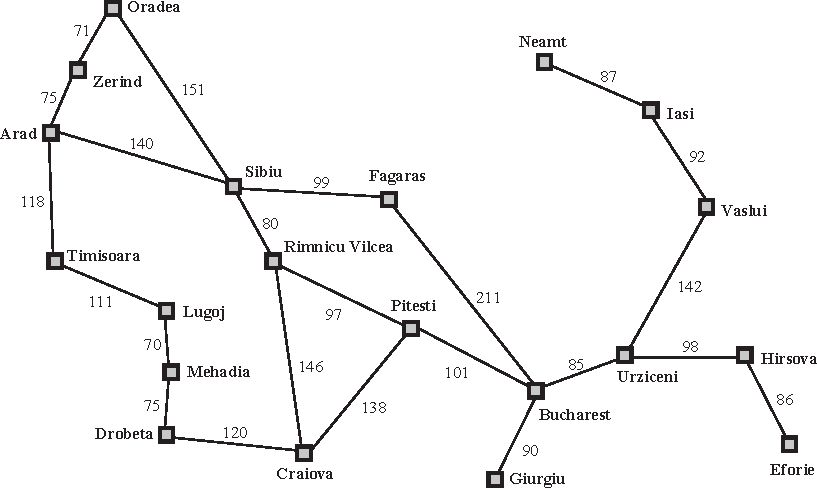
\includegraphics[scale=1]{Romania Map}
\caption{A simplified road map of part of Romania. Numbers are distances.}\label{RomaniaMap}
\end{figure}

\section{Solving problems with agents}
The simplest agents discussed previously were the reflex agents, which base their actions on a direct mapping from states to actions. Such agents cannot operate well in environments for which this mapping would be too large to store and would take too long to learn. Goal-based agents, on the other hand, consider future actions and the desirability of their outcomes.
This chapter describes one kind of goal-based agent called a problem-solving agent.

Our discussion of problem solving begins with precise definitions of problems and their solutions and give several examples to illustrate these definitions. We then describe several general-purpose search algorithms that can be used to solve these problems.

We will see several uninformed search algorithms that are given no information about the problem other than its definition. Although some of these algorithms can solve any solvable problem, none of them can do so efficiently. Informed search algorithms, on the other hand, can do quite well given some guidance on where to look for solutions.
\subsection{Formulation of a problem}
\textbf{Goal formulation}, based on the current situation and the agent’s performance measure, is the first step in problem solving.

\textbf{Problem formulation} is the process of deciding what actions and states to consider, given a goal. We discuss this process in more detail later.

We make several \textcolor{CadetBlue!90}{\textbf{assumption}}: a static, fully accessible, discrete and deterministic environment.Under these assumptions, the \textbf{Solution} to any problem is a fixed sequence of actions.
The process of looking for a sequence of actions that reaches the goal is called \textbf{Search}.
A \textbf{Search Algorithm} takes a problem as input and returns a solution in the form of an action sequence. Once a solution is found, the actions it recommends can be carried out. This is called the \textbf{Execution Phase}.

\subsection{Well-defined problems and solutions}
A problem can be defined formally by five components:
\begin{itemize}
  \item The \textbf{Initial State} that the agent starts in.
  \item A \textbf{description of the possible actions} "a" available to the agent. Given a particular state "s", we say that each of these actions is \textcolor{CadetBlue!90}{\textbf{applicable}} in s.
    ACTIONS(s) returns the set of actions that can be executed in s.
  \item A description of what each action does; the formal name for this is the \textbf{Transition Model}, specified by a function $RESULT(s, a)$ that returns the state that results from doing action a in state s. We also use the term successor to refer to any state reachable from a given state by a single action.
\[RESULT(In(Arad),Go(Zerind)) = In(Zerind)\]
  Together, the Initial State, actions, and transition model implicitly define the \textcolor{CadetBlue!90}{\textbf{State Space}} of the problem the set of all states reachable from the initial state by any sequence of actions. The state space forms a directed network or \textcolor{CadetBlue!90}{\textbf{graph}} in which the \textcolor{CadetBlue!90}{\textbf{nodes}} are states and the \textcolor{CadetBlue!90}{\textbf{links}} between nodes are actions.
  A \textcolor{CadetBlue!90}{\textbf{path}} in the state space is a sequence of states connected by a sequence of actions.
  \item The \textbf{goal test}, which determines whether a given state is a goal state. Sometimes there is an explicit set of possible goal states, and the test simply checks whether the given state is one of them.
  \item A \textbf{path cost function} that assigns a numeric cost to each path. The problem-solving agent chooses a cost function that reflects its own performance measure.
\end{itemize}

%\begin{itemize}
%  \item Initialstate: I am in Timisoara
%  \item Possible actions(action, successor): (go Arad, in Arad), (go Lugoj, in Lugoj)
%  \item Goal test: in Bucarest?
%  \item Path costfrom x to y by the action a: $c(x,a,y)>=0$
%  \item Optimalsolution: the solutionhavingthe lowestcost
%\end{itemize}

\subsection{Search algorithm}

\subsubsection{Search Algorithm structure and the State Space}
A solution is an action sequence, so search algorithms work by considering various possible action sequences.
The possible action sequences starting at the initial state form a search tree with the initial state at the root; the branches are actions and the nodes correspond to states in the state space of the problem.

In this list there are the main components of a state space together with the relation between them:
\begin{itemize}
  \item Path - Path refers to the sequence of nodes along the edges of a tree.

  \item Root - The node at the top of the tree is called root. There is only one root per tree and one path from the root node to any node.

  \item Parent node - Any node except the root node has one edge upward to a node called parent.

  \item Child node - The node below a given node connected by its edge downward is called its child node.

  \item Leaf node - The node which does not have any child node is called the leaf node. Leaf node can be expanded and then become Parent Node if they have children node, or remain Leaf node if they haven't.

  \item Subtree - Subtree represents the descendants of a node.

  \item Visiting - Visiting refers to checking the value of a node when control is on the node.

  \item Traversing - Traversing means passing through nodes in a specific order.

  \item Depth or Levels - Level of a node represents the generation of a node. If the root node is at level 0, then its next child node is at level 1, its grandchild is at level 2, and so on.

  \item Keys - Key represents a value of a node based on which a search operation is to be carried out for a node.

  \item Frontier - The set of all leaf nodes available for expansion at any given point is called the frontier.

  \item Fringe - Collection of nodes generated but not yet expanded
\end{itemize}
\begin{figure}[h!]
\centering
\subfloat[][\emph{Search Tree}]
{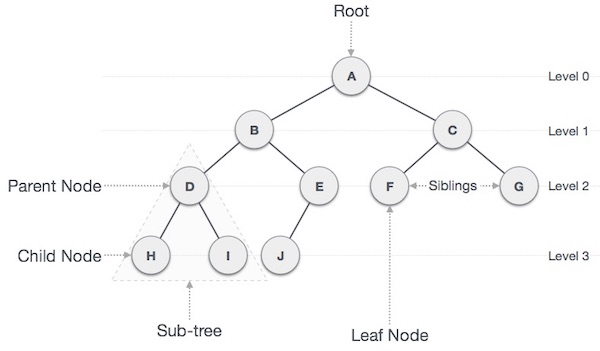
\includegraphics[width=.80\textwidth]{binary_tree.jpg}}
\caption{Search Tree}
\label{fig:Search Tree}
\end{figure}

Search algorithms follows a simple structure:
\begin{enumerate}
  \item The root node of the tree corresponds to the initial state, $In(s=root)$. The first step is to test whether this is a goal state.
  \item Then we need to consider taking various actions:
  We do this by \textbf{expanding} the current state; that is, applying each legal action to the current state, thereby \textbf{generating} a new set of states which are linked by branches to the current (parent node) state leading to new child node.
  \item Now we must apply the specific iterative algorithm that is chosen for the problem and then move to the child node given by the algorithm.
  \item The process of expanding nodes on the frontier continues until either a solution is found or there are no more states to expand.
\end{enumerate}

This is the general \textbf{TREE-SEARCH} algorithm.

Search algorithms all share this basic structure; they vary primarily according to how they choose which state to expand next the so-called \textbf{search strategy}.

An exception is given if there is a repeated state in the search tree such that it can generate a loopy path that can become infinite if we don't take precautions.

The way to avoid exploring redundant paths is to remember where one has been. To do this, we augment the \textbf{TREE-SEARCH} algorithm with a data structure called the \textbf{explored set} (also known as the \textbf{closed list}), which remembers every expanded node. Newly generated nodes that match previously generated nodes ones in the explored set or the frontier can be discarded instead of being added to the frontier. The new algorithm, called \textbf{GRAPH-SEARCH}. The specific algorithms in this chapter draw on this general design.
Clearly, the search tree constructed by the GRAPH-SEARCH algorithm contains at most one copy of each state, so we can think of it as growing a tree directly on the state-space graph. The algorithm has another nice property: the frontier separates the state-space graph into the explored region and the unexplored region, so that every path fromthe initial state to an unexplored state has to pass through a state in the frontier.
\paragraph{Difference between TREE-SEARCH and GRAPH-SEARCH}

Firstly, we have to understand that the underlying problem (or search space) is almost always represented as a graph (although the underlying graph may not contain cycles, so it may represent a tree). So, the difference between tree-search and graph-search is not whether the problem is a tree (a special kind of graph), or a general graph!

The distinction is, instead, how we are traversing the search space (represented as a graph) to search for our goal state and whether we are using an additional list (called the closed list) or not.

So, the basic differences are:
\begin{enumerate}
  \item In the case of a graph search, we use a list, called the closed list (also called explored set), to keep track of the nodes that have already been visited and expanded, so that they are not visited and expanded again.

  \item In the case of a tree search, we do not keep this closed list. Consequently, the same node can be visited multiple (or even infinitely many) times, which means that the produced tree (by the tree search) may contain the same node multiple times.
\end{enumerate}


The advantage of graph search obviously is that, if we finish the search of a node, we will never search it again. On the other hand, the tree search can visit the same node multiple times.

The disadvantage of graph search is that it uses more memory (which we may or may not have) than tree search. This matters because graph search actually has exponential memory requirements in the worst case, making it impractical without either a really good search heuristic or an extremely simple problem.
\subsubsection{Infrastructure for search algorithms Node - Function and Queue}
Search algorithms require a data structure to keep track of the search tree that is being constructed.
For each node n of the tree, we have a structure (usually a class) that contains five components:
\begin{itemize}
  \item n.STATE: the state in the state space to which the node corresponds;
  \item n.PARENT: the node in the search tree that generated this node;
  \item n.ACTION: the action that was applied to the parent to generate the node (n-1,a,n);
  \item n.PATH-COST: the cost, traditionally denoted by $g(n)= \sum_{i=1}^{n} c(i-1, a_{i}, i)$, of the path from the initial state to the node, as indicated by the parent pointers.
\end{itemize}
The function CHILD-NODE takes a parent node and an action
and returns the resulting child node.

These pointers also allow the solution path to be
extracted when a goal node is found; we use the SOLUTION function to return the sequence of actions obtained by following parent pointers back to the root.

Up to now, we have not been very careful to distinguish between nodes and states, but in writing detailed algorithms it’s important to make that distinction. A node is a bookkeeping data structure used to represent the search tree. A state corresponds to a configuration of the world.

Now that we have nodes, we need somewhere to put them. The frontier needs to be stored in such a way that the search algorithm can easily choose the next node to expand QUEUE according to its preferred strategy. The appropriate data structure for this is a queue. The operations on a queue are as follows:
\begin{itemize}
  \item EMPTY?(queue) returns true only if there are no more elements in the queue.
  \item POP(queue) removes the first element of the queue and returns it.
  \item INSERT(element, queue) inserts an element and returns the resulting queue.
\end{itemize}

Queues are characterized by the order in which they store the inserted nodes. Three common variants are the first-in, first-out or FIFO queue, which pops the oldest element of the queue;
the last-in, first-out or LIFO queue (also known as a stack), which pops the newest element of the queue; and the priority queue, which pops the element of the queue with the highest
priority according to some ordering function.

\subsubsection{Problem-Solving performance}
Measuring problem-solving performance before we get into the design of specific search algorithms, we need to consider the criteria that might be used to choose among them.
We can evaluate an algorithm’s performance in four ways:
\begin{itemize}
  \item COMPLETENESS : Is the algorithm guaranteed to find a solution when there is one?
  \item OPTIMALITY: Does the strategy find the optimal solution? An optimal solution has the lowest path cost among all solutions.
  \item TIME COMPLEXITY: How long does it take to find a solution?
  \item SPACE COMPLEXITY: How much memory is needed to perform the search?
\end{itemize}

Time and space complexity are always considered with respect to some measure of the problem difficulty. In theoretical computer science, the typical measure is the size of the state space graph, $|V| + |E|$, where V is the set of vertices (nodes) of the graph and E is the set of edges (links).

This is appropriate when the graph is an explicit data structure that is input to the search program. (The map of Romania is an example of this.)
In AI, the graph is often represented implicitly by the initial state, actions, and transition model and is frequently infinite.
For these reasons, \textcolor{CadetBlue!90}{\textbf{complexity is expressed in terms of three quantities}}: \textbf{b}, the branching factor or maximum number of successors of any node; \textbf{d}, the depth of the shallowest goal node (i.e., the number of steps along the path from the root); and \textbf{m}, the maximum length of any path in the state space. Time is often measured in terms of the number of nodes generated during the search, and space in terms of the maximum number of nodes stored in memory.
For the most part, we describe time and space complexity for search on a tree; for a graph, the answer depends on how “redundant” the paths in the state space are.
To assess the effectiveness of a search algorithm, we can consider just the search cost which typically depends on the time complexity but can also include a term for memory usage or we can use the total cost, which combines the search cost and the path cost of the solution found.

Regarding space complexity: for any kind of graph search, which stores every expanded node in the explored set, the space complexity is always within a factor of b of the time complexity.

\section{Search algorithms}
This section covers several search strategies that come under the heading of \textbf{uninformed search} (also called blind search). The term means that the strategies have no additional information about states beyond that provided in the problem definition. All they can do is generate successors and distinguish a goal state from a non-goal state.
All search strategies are distinguished by the order in which nodes are expanded. Strategies that know whether one non-goal state is “more promising” than another are called \textbf{informed search} or \textbf{heuristic search} strategies.
\subsection{Uninformed Search Algorithms}
\subsubsection{Breadth-first search}
Breadth-first search (ricerca in ampiezza) is a simple strategy in which the root node is expanded first, then all the successors of the root node are expanded next, then their successors, and so on. In general,
all the nodes are expanded at a given depth in the search tree before any nodes at the next level are expanded.

It is complete if the shallowest (più superficiale) goal node is at some finite depth d, breadth-first search will eventually find it after generating all shallower nodes (provided the branching factor b is finite). Note that as soon as a goal node is generated, we know it is the shallowest goal node because all shallower nodes must have been generated already and failed the goal test. Now, the shallowest goal node is not necessarily the optimal one; technically, breadth-first search is optimal if the path cost is a nondecreasing function of the depth of the node. The most common such scenario is that all actions have the same cost.

The root of the search tree generates b nodes at the first level, each of which generates b more nodes, for a total of b 2 at the second level. Each of these generates b more nodes, yielding b 3 nodes at the third level, and so on. Now suppose that the solution is at depth d. In the worst case, it is the last node generated at that level.

Then the total number of nodes generated is
\[b + b^2 + b^3 + \dots + b^d
 = \mathcal{O}(b^d)\]

As for space complexity: for any kind of graph search, which stores every expanded node in the explored set, the space complexity is always within a factor of b of the time complexity. For breadth-first graph search in particular, every node generated remains in memory.
There will be $\mathcal{O}(b^{d-1})$ nodes in the explored set and $\mathcal{O}(b^d)$ nodes in the frontier, so the space complexity is $\mathcal{O}(b^d)$, i.e., it is dominated by the size of the frontier.
 Switching to a tree search would not save much space, and in a state space with many redundant paths, switching could cost a great deal of time.
An exponential complexity bound such as $\mathcal{O}(b^d)$ is scary. It lists, for various values of the solution depth d, the time and memory required for a breadthfirst search with branching factor $b = 10$. The table \textcolor{CadetBlue!90}{\textbf{assumes that 1 million nodes can be generated per second}} and that a node requires $1000$ bytes of storage. Many search problems fit roughly within these assumptions (give or take a factor of $100$) when run on a modern personal computer.
\begin{figure}[h!]
\centering
\subfloat[][\emph{Breadth Search}]
{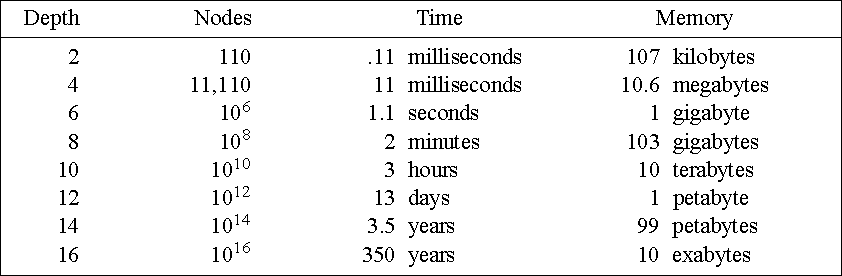
\includegraphics[width=.80\textwidth]{Breadth.pdf}}
\caption{Breadth Search}
\label{fig:Breadth Search}
\end{figure}

\paragraph{General conclusion for uninformed search:}
First, the memory requirements are a bigger problem for breadth-first search than is the execution time.
In general, exponential-complexity search problems
cannot be solved by uninformed methods for any but the smallest instances.
\subsubsection{Uniform-cost search}
When all step costs are equal, breadth-first search is optimal because it always expands the shallowest unexpanded node. By a simple extension, we can find an algorithm that is optimal with any step-cost function. Instead of expanding the shallowest node, uniform-cost search expands the node n with the lowest path cost g(n). This is done by storing the frontier as a priority queue ordered by g.
In addition to the ordering of the queue by path cost, there are two other significant differences from breadth-first search. The first is that the goal test is applied to a node when it is selected for expansion, rather than when it is first generated.
The second difference is that a test is added in case a better path is found to a node currently on the frontier.
It is easy to see that uniform-cost search is optimal in general.
Uniform-cost search does not care about the number of steps a path has, but only about their total cost. Therefore, it will get stuck in an infinite loop if there is a path with an infinite sequence of zero-cost action.

Uniform-cost search is guided by path costs rather than depths, so its complexity is not easily characterized in terms of b and d. Instead, let $C^*$ be the cost of the optimal solution, and assume that every action costs at least $\epsilon$. Then the algorithm’s worst-case time and space complexity is $\mathcal{O}(b^{1+\frac{C^*}{\epsilon}})$.
\subsubsection{Depth-first search}
Depth-first search always expands the deepest node in the current frontier of the search tree.
The search proceeds immediately to the deepest level of the search tree, where the nodes have no successors. As those nodes are expanded, they are dropped from the frontier, so then the search “backs up” to the next deepest node that still has unexplored successors.
Whereas breadth-first-search uses a FIFO queue, depth-first search uses a LIFO queue.
A LIFO queue means that the most recently generated node is chosen for expansion. This must be the deepest unexpanded node because it is one deeper than its parent which, in turn, was the deepest unexpanded node when it was selected.


A variant of depth-first search called backtracking search uses still less memory. In backtracking, only one successor is generated at a time rather than all successors; each partially expanded node remembers which successor to generate next. In this way, only $\mathcal{O}(m)$ memory is needed rather than $\mathcal{O}(bm)$. Backtracking search facilitates yet another memory-saving (and time-saving) trick: the idea of generating a successor by modifying the current state description directly rather than copying it first. This reduces the memory requirements to just one state description and $\mathcal{O}(m)$ actions. For this to work, we must be able to undo each modification when we go back to generate the next successor. For problems with large state descriptions, such as robotic assembly, these techniques are critical to success.

\subsubsection{Depth-limited Search}

The embarrassing failure of depth-first search in infinite state spaces can be alleviated by supplying depth-first search with a predetermined depth limit $\ell$. That is, nodes at depth $\ell$ are  treated as if they have no successors. This approach is called depth-limited search. The depth limit solves the infinite-path problem. Unfortunately, it also introduces an additional source of incompleteness if we choose $\ell < d$, that is, the shallowest goal is beyond the depth limit. (This is likely when d is unknown.) Depth-limited search will also be nonoptimal if we choose $\ell > d$. Its time complexity is $\mathcal{0}(b^{\ell})$ and its space complexity is $\mathcal{O} (b\ell)$.
 Depth-first search can be viewed as a special case of depth-limited search with $\ell=\infty$.

\subsubsection{Iterative Deepening search}
 Iterative Deepening search (or iterative deepening depth-first search) is a general strategy, often used in combination with depth-first tree search, that finds the best depth limit. It does this by gradually increasing the limit first 0, then 1, then 2, and so on—until a goal is found. This will occur when the depth limit reaches d, the depth of the shallowest goal node.

 In general, iterative deepening is the preferred uninformed search method when the search space is large and the depth of the solution is not known.

 \subsubsection{Bidirectional Search}
 The idea behind bidirectional search is to run two simultaneous searches—one forward from the initial state and the other backward from the goal—hoping that the two searches meet in the middle. The motivation is that $b^{d/2} + b^{d/2}$ is much less than $b^d$, or in the figure, the area of the two small circles is less than the area of one big circle centered on the start and reaching to the goal.
Bidirectional search is implemented by replacing the goal test with a check to see whether the frontiers of the two searches intersect; if they do, a solution has been found.
\subsubsection{Comparison}
\begin{figure}[h!t]
\centering
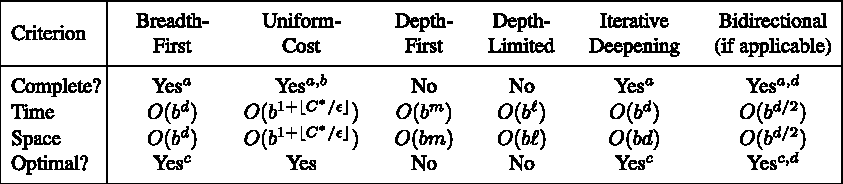
\includegraphics[width=.80\textwidth]{Comparison.pdf}
\caption{ Evaluation of tree-search strategies. $b$ is the branching factor; $d$ is the depth of the shallowest solution; $m$ is the maximum depth of the search tree; $l$ is the depth limit.
Superscript caveats are as follows: $^{a}$ complete if $b$ is finite; $^{b}$ complete if step costs $\geq \epsilon$ for positive $\epsilon$; $^{c}$ optimal if step costs are all identical; $^{d}$ if both directions use breadth-first search.}
\label{fig:Strategies comparison}
\end{figure}

\subsection{Informed search algorithm}
This section shows how an informed \textbf{INFORMED SEARCH} search strategy—one that uses problem-specific knowledge beyond the definition of the problem itself can find solutions more efficiently than can an uninformed strategy.
The general approach we consider is called \textbf{best-first search}. Best-first search is an instance of the general TREE-SEARCH or GRAPH-SEARCH algorithm in which a node is selected for expansion based on an \textbf{evaluation function}, f(n). The evaluation function is construed as a cost estimate, so the node with the lowest evaluation is expanded first. The implementation of best-first graph search is identical to that for uniform-cost search, except for the use of f instead of g to order the priority queue.
The choice of f determines the search strategy. Most best-first algorithms include as a component of f a \textbf{heuristic function}, denoted h(n):

\[h(n) = \text{estimated cost of the cheapest path from the state at node n to a goal state.}\]

(Notice that h(n) takes a node as input, but, unlike g(n), it depends only on the state at that node.)
Heuristic functions are the most common form in which additional knowledge of the problem is imparted to the search algorithm.

For now, we consider them to be arbitrary, non negative, problem-specific functions, with one constraint: \textbf{if n is a goal node, then h(n)=0}. The remainder of this section covers two ways to use heuristic information to guide search.

\subsubsection{Greedy best-first search}
Greedy best-first search tries to expand the node that is closest to the goal, on the grounds that this is likely to lead to a solution quickly. Thus, it evaluates nodes by using just the heuristic function; that is, f(n) = h(n).

We use the \textbf{straight line distance heuristic}, which we will call $h_{SLD}$.

The algorithm is called “greedy”—at each step it tries to get as close to the goal as it can.
Greedy best-first tree search is incomplete even in a finite state space, much like depth-first search and also it is not optimal.
\subsubsection{A\text{*} search: Minimizing the total estimated solution cost}
The most widely known form of best-first search is called A\text{*} (pronounced “A-star search”). It evaluates nodes by combining $g(n)$, the cost to reach the node, and $h(n)$, the cost to get from the node to the goal:
$f(n) = g(n) + h(n)$.
Since $g(n)$ gives the path cost from the start node to node n, and $h(n)$ is the estimated cost of the cheapest path from n to the goal, we have:
\[f(n) = \text{estimated cost of the cheapest solution through n}\]
Thus, if we are trying to find the cheapest solution, a reasonable thing to try first is the node with the lowest value of $g(n) + h(n)$. It turns out that this strategy is more than just reasonable: provided that the heuristic function $h(n)$ satisfies certain conditions, A\text{*} search is both complete and optimal. The algorithm is identical to Uniform-cost search except that A\text{*} uses $g + h$ instead of $g$.

\paragraph{Conditions for optimality: Admissibility and consistency}
The first condition we require for \textbf{optimality} is that h(n) be an admissible heuristic. An admissible heuristic is one that never overestimates the cost to reach the goal. Because g(n) is the actual cost to reach n along the current path, and f(n)=g(n) + h(n), we have as an immediate consequence that f(n) never overestimates the true cost of a solution along the current path through n.
Admissible heuristics are by nature optimistic because they think the cost of solving
the problem is less than it actually is.
An obvious example of an admissible heuristic is the straight-line distance $h_{LSD}$

A second, slightly stronger condition called  \textbf{consistency} (or sometimes monotonicity) is required only for applications of A\text{*} to graph search.
A heuristic h(n) is consistent if, for every node n and every successor n' of n generated by any action a, the estimated cost of reaching the goal from n is no greater than the step cost of getting to n' plus the estimated cost of reaching the goal from n': $h(n) \leq c(n, a, n') + h(n')$.

This is a form of the general \textcolor{CadetBlue!90}{\textbf{triangle inequality}}, which stipulates that each side of a triangle cannot be longer than the sum of the other two sides. Here, the triangle is formed by n, n', and the goal $G_n$ closest to n. For an admissible heuristic, the inequality makes perfect sense:
if there were a route from n to $G_n$ via n' that was cheaper than h(n), that would violate the
property that h(n) is a lower bound on the cost to reach $G_n$.
It is fairly easy to show that \textcolor{CadetBlue!90}{\textbf{every consistent heuristic is also admissible}} as follow from the demonstration:
\[    h(n) \leq c(n, a_{1}, n_{1}) + h(n_{1})\leq  c(n, a_{1}, n_{1}) +  c(n_{1}, a_{2}, n_{2}) + h(n_{2}) \leq \dots\]
\[\dots \leq c(n, a_{1}, n_{1}) + \dots + c(n_{d-1}, a_{d}, G^{*}) + h(G^{*})=C(n,G^{*})\]
Consistency is therefore a stricter requirement than admissibility, but one has to work quite hard to construct heuristics that are admissible but not consistent.
\begin{itemize}
    \item Admissible implies complete
    \item Consistent implies complete and optimal
\end{itemize}
Exercise: Prove that if a heuristic is consistent, it must be admissible. Construct an admissible
heuristic that is not consistent.

\paragraph{Optimality of A*}
As we mentioned earlier, A* has the following properties: the tree-search version of A\text{*} is
optimal if $h(n)$ is admissible, while the graph-search version is optimal if $h(n)$ is consistent.
We show the second of these two claims since it is more useful. The argument essentially mirrors the argument for the optimality of uniform-cost search, with g replaced by f just as in the A\text{*} algorithm itself.
The first step is to establish the following: if h(n) is consistent, then the values of f(n) along any path are nondecreasing. The proof follows directly from the definition of consistency. Suppose n' is a successor of n; then $g(n')=g(n) + c(n, a, n')$ for some action a, and we have 
\begin{equation}
    f(n') = g(n') + h(n') = g(n) + c(n, a, n') + h(n') \geq g(n) + h(n) = f(n)
\end{equation}

The next step is to prove that whenever A\text{*} selects a node n for expansion, the optimal path to that node has been found. Were this not the case, there would have to be another frontier node n' on the optimal path from the start node to n, because f is nondecreasing along any path, n' would have lower f-cost than n and would have been selected first.
Because f is nondecreasing along any path, n' would have lower f-cost than n and would have been selected first.\footnote{See figure 3.9 pag. 78 \cite{RusselNorvig:2009dg} for the separation properties of graph}


\paragraph{Inventing Heuristic function}
code: 8-puzzle game\\

Queen game\\

see crystal quest, a game for machintosh using greedy algorithm in the demo mode

\paragraph{The effect of heuristic accuracy on performance}
One way to characterize the quality of a heuristic is the effective \textcolor{CadetBlue!90}{\textbf{branching factor}} \textbf{b\text{*}}. If the total number of nodes generated by A\text{*} for a particular problem is N and the solution depth is d, then b\text{*} is the branching factor that a uniform tree of depth d would have to have in order to contain $N + 1$ nodes. Thus, $N + 1 = 1+b\text{*} + (b\text{*})^{2} +\dots+ (b\text{*})^d$.
For example, if A\text{*} finds a solution at depth 5 using 52 nodes, then the effective branching factor is 1.92. The effective branching factor can vary across problem instances, but usually it is fairly constant for sufficiently hard problems. (The existence of an effective branching factor follows from the result, mentioned earlier, that the number of nodes expanded by A\text{*} grows exponentially with solution depth.) Therefore, experimental measurements of b* on a small set of problems can provide a good guide to the heuristic’s overall usefulness. A welldesigned heuristic would have a value of b\text{*} close to 1, allowing fairly large problems to be solved at reasonable computational cost.

\paragraph{Learning heuristics from experience}
Hints on generating a heuristic function using neural network.

\section{Local Search}
In the last Section we addressed a single category of problems: observable, deterministic, known environments where the solution is a sequence of actions. In this chapter, we look at what happens when these \textcolor{CadetBlue!90}{\textbf{assumptions are relaxed}}.
The answer to this problem is given by \textbf{local search} in the state space, evaluating and modifying one or more current states rather than systematically exploring paths from an initial state.
These algorithms are suitable for problems in which all that matters is the solution state, not the path cost to reach it. The family of local search algorithms includes methods inspired by statistical physics (\textbf{simulated annealing}) and evolutionary biology (\textbf{genetic algorithms}).

Then, we examine what happens when we relax the assumptions of determinism and observability. The key idea is that if an agent cannot predict exactly what percept it will receive, then it will need to consider what to do under each contingency that its percepts may reveal. With partial observability, the agent will also need to keep track of the states it might be in.
\paragraph{Local search:}
The search algorithms that we have seen so far are designed to explore search spaces systematically.
This systematicity is achieved by keeping one or more paths in memory and by recording which alternatives have been explored at each point along the path.
In many problems, however, the path to the goal is irrelevant. For example, in the 8-queens problem, what matters is the final configuration of queens, not the order in which they are added. 

If the path to the goal does not matter, we might consider a different class of algorithms, ones that do not worry about paths at all. Local search algorithms operate using a single \textbf{current node} (rather than multiple paths) and generally move only to neighbors of that node. Typically, the paths followed by the search are not retained.
Although local search algorithms are not systematic, they have two key advantages: 
\begin{enumerate}
    \item they use very little memory—usually a constant amount;
    \item they can often find reasonable solutions in large or infinite (continuous) state spaces for which systematic algorithms are unsuitable.
\end{enumerate}
In addition to finding goals, local search algorithms are useful for solving \textbf{pure optimization problems}, in which the aim is to find the best state according to an \textbf{objective function}. Many optimization problems do not fit the “standard” search model introduced. 
For example, nature provides an objective function that Darwinian evolution could be seen as attempting to optimize, but there is no “goal test” and no “path cost” for this problem.
To understand local search, we find it useful to consider the state-space landscape. A landscape has both “location” (defined by the state) and “elevation” (defined by the value of the heuristic cost function or objective function). If elevation corresponds to \textbf{GLOBAL MINIMUM} cost, then the aim is to find the lowest valley: a global minimum; if elevation corresponds \textbf{GLOBAL MAXIMUM} to an objective function, then the aim is to find the highest peak—a global maximum. (You can convert from one to the other just by inserting a minus sign.) Local search algorithms explore this landscape. A \textbf{complete} local search algorithm always finds a goal if one exists;an \textbf{optimal} algorithm always finds a global minimum/maximum.

\begin{figure}[h!t]
\centering
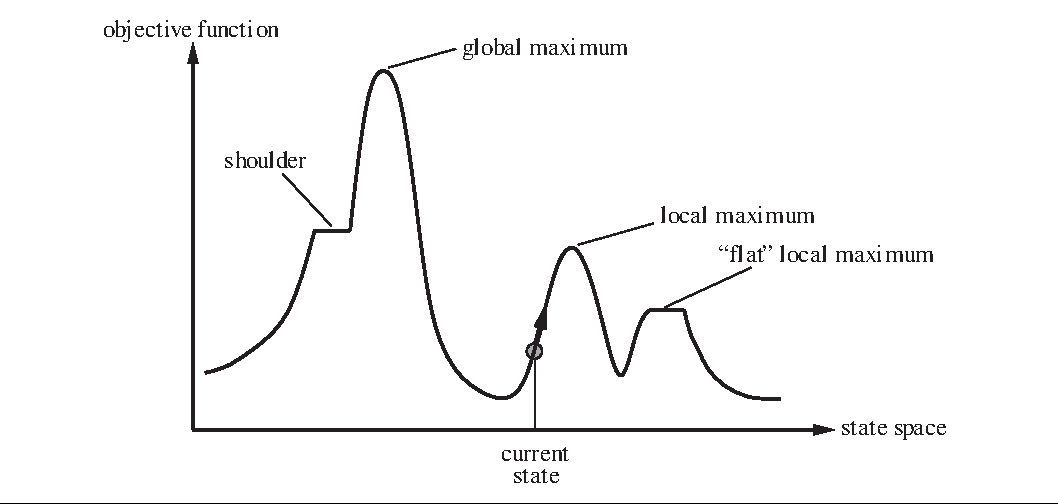
\includegraphics[scale=0.8]{Maxmin.pdf}
\caption{A one-dimensional state-space landscape in which elevation corresponds to the
objective function. The aim is to find the global maximum. Hill-climbing search modifies
the current state to try to improve it, as shown by the arrow. The various topographic features
are defined in the text.}
\end{figure}

\subsection{Strategies for local search}
\begin{itemize}
    \item Hill-climbing search 
    \item Montecarlo technique, simulated annealing: random walk and down-hill moves
    \item Local beam search: generates all successors of k replica, then selects the best k successors from the complete list
    \item Stochastic beam search: chooses randomly k successors from the complete list, with probability increasing with its value
    \item Genetic algorithms: combines two parents and tries to mimic natural selection
\end{itemize}
\subsection{Hill-climbing search or Greedy local search}
It is simply a loop that continually moves in the direction of increasing value—that is, uphill. It
terminates when it reaches a “peak” where no neighbor has a higher value. The algorithm
does not maintain a search tree, so the data structure for the current node need only record
the state and the value of the objective function. Hill climbing does not look ahead beyond
the immediate neighbors of the current state. This resembles trying to find the top of Mount
Everest in a thick fog while suffering from amnesia.
To illustrate hill climbing, we will use the 8-queens problem.
Local search algorithms typically use a complete-state formulation: each state contain all the configuration of the system. Hill climbing is sometimes called greedy local search because it grabs a good neighbor state without thinking ahead about where to go next. Although greed is considered one of the seven deadly sins, it turns out that greedy algorithms often perform quite well.
\\
Unfortunately, hill climbing often gets stuck for the following reasons:
\begin{itemize}
\item Local maximum: a local maximum is a peak that is higher than each of its neighboring
states but lower than the global maximum. Hill-climbing algorithms that reach the
vicinity of a local maximum will be drawn upward toward the peak but will then be
stuck with nowhere else to go.
\item Ridges: a ridge is shown in Figure \ref{ridges}. Ridges result in a sequence of local maxima
that is very difficult for greedy algorithms to navigate.
\item Plateaux: a plateau is a flat area of the state-space landscape. It can be a flat local maximum, from which no uphill exit exists, or a shoulder, from which progress is possible. A hill-climbing search might get lost on the plateau.
\end{itemize}
In each case, the algorithm reaches a point at which no progress is being made.
The algorithm may reaches a plateau where the best successor has the same value as the current state. Might it not be a good idea to keep going—to allow a
sideways move in the hope that the plateau is really a shoulder? The answer is usually yes, but we must take care. If we always allow sideways moves when there are no uphill moves, an infinite loop will occur whenever the algorithm reaches a flat local maximum that is not a shoulder. One common solution is to put a limit on the number of consecutive sideways moves allowed.
Many variants of hill climbing have been invented.
\begin{figure}[h!t]
\centering
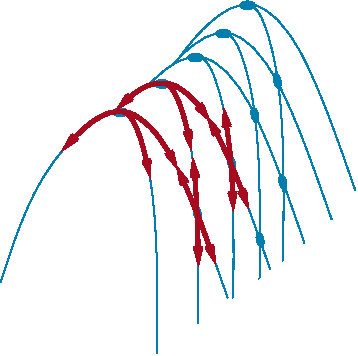
\includegraphics[scale=0.8]{Ridges.pdf}
\caption{Illustration of why ridges cause difficulties for hill climbing. The grid of states
(dark circles) is superimposed on a ridge rising from left to right, creating a sequence of local
maxima that are not directly connected to each other. From each local maximum, all the
available actions point downhill.}\label{ridges}
\end{figure}

\paragraph{Random-restart hill climbing} is a variant of the technique. 
It conducts a series of hill-climbing searches from randomly generated initial states, until a goal is found. It is trivially complete with probability approaching 1, because it will eventually generate a goal state as the initial state. If each hill-climbing search has a probability p of success, then the expected number of restarts required is 1/p.

\subsection{Simulated Annealing}
A hill-climbing algorithm that never makes “downhill” moves toward states with lower value (or higher cost) is guaranteed to be incomplete, because it can get stuck on a local maximum.
In contrast, a purely random walk—that is, moving to a successor chosen uniformly at random from the set of successors—is complete but extremely inefficient. Therefore, it seems reasonable to try to combine hill climbing with a random walk in some way that yields
both efficiency and completeness.
\textbf{Simulated annealing} is such an algorithm. In metallurgy, \textbf{annealing} is the process used to temper or harden metals and glass by heating them to a high temperature and then gradually cooling them, thus allowing the material to reach a low energy crystalline state. To explain simulated annealing, we switch our point of view from hill climbing to \textbf{gradient descent} and imagine the task of getting a ping-pong ball into the deepest crevice in a bumpy surface. If we just let the ball roll, it will come to rest at a local minimum. If we shake the surface, we can bounce the ball out of the local minimum. The trick is to shake just hard enough to bounce the ball out of local minima but not hard enough to dislodge it from the global minimum. The simulated-annealing solution is to start by shaking hard (i.e., at a high temperature) and then gradually reduce the intensity of the shaking (i.e., lower the temperature).
The innermost loop of the simulated-annealing algorithm is quite similar to hill climbing. Instead of picking the best move, however, it picks a random move. If the move
improves the situation, it is always accepted. Otherwise, the algorithm accepts the move with some probability less than 1. The probability decreases exponentially with the “badness” of the move—the amount $\Delta E$ by which the evaluation is worsened.
The probability also decreases as the “temperature” T goes down: “bad” moves are more likely to be allowed at the start when T is high, and they become more unlikely as T decreases. If the schedule lowers T slowly enough, the algorithm will find a global optimum with probability approaching 1.

\subsubsection{Solving again Travelling Salesman DA COMPLETARE MATIAS}
Pag. 549 Numerical Recipes Approfondire.
Pag 551 Traveling Salesman

\subsection{Local Beam Search}
Keeping just one node in memory might seem to be an extreme reaction to the problem of
memory limitations. The local beam search algorithm\footnote{Local beam search is an adaptation of \textbf{beam search}, which is a path-based algorithm.} keeps track of k states rather than just one. It begins with k randomly generated states. At each step, all the successors of all k states are generated. If any one is a goal, the algorithm halts. Otherwise, it selects the k best successors from the complete list and repeats.
At first sight, a local beam search with k states might seem to be nothing more than running k random restarts in parallel instead of in sequence. In fact, the two algorithms are quite different. In a random-restart search, each search process runs independently of the others. In a local beam search, useful information is passed among the parallel search threads. In effect, the states that generate the best successors say to the others, “Come over here, the grass is greener!” The algorithm quickly abandons unfruitful searches and moves its resources to where the most progress is being made. In its simplest form, local beam search can suffer from a lack of diversity among the k states—they can quickly become concentrated in a small region of the state space, making the search little more than an expensive version of hill climbing. 

A variant called \textbf{stochastic beam search}, analogous to stochastic hill climbing, helps alleviate this problem. Instead of choosing the best k from the the pool of candidate successors, stochastic beam search chooses k successors at random, with the probability of choosing a given successor being an increasing function of its value. Stochastic beam search bears some resemblance to the process of natural selection, whereby the “successors” (offspring) of a “state” (organism) populate the next generation according to its “value” (fitness).


\subsection{Genetic algorithm}
A \textbf{genetic algorithm} (or GA) is a variant of stochastic beam search in which successor states are generated by combining two parent states rather than by modifying a single state. The analogy to natural selection is the same as in stochastic beam search, except that now we are dealing with sexual rather than asexual reproduction.
Like beam searches, GAs begin with a set of k randomly generated states, called the \textbf{population}. Each state, or \textbf{individual}, is represented as a string over a finite alphabet—most commonly, a string of 0s and 1s. For example, an 8-queens state must specify the positions of 8 queens, each in a column of 8 squares, and so requires $8\times \log{2 8}=24$ bits. Alternatively, the state could be represented as 8 digits, each in the range from 1 to 8.
\begin{figure}[h!]
\centering
{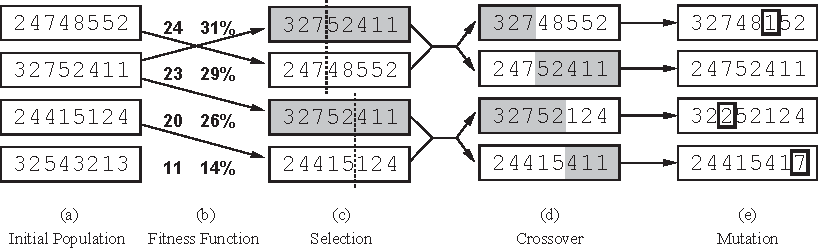
\includegraphics[width=.80\textwidth]{Genetic Algorithm (1).pdf}}
\caption{}
\label{fig:geneticalgorithm1}
\end{figure}

\begin{figure}[h!]
\centering
{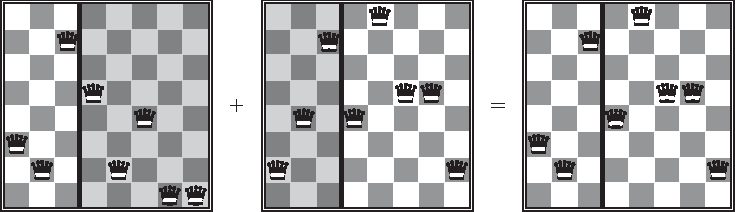
\includegraphics[width=.80\textwidth]{Genetic Algorithm (2).pdf}}
\caption{}
\label{fig:geneticalgorithm2}
\end{figure}
The production of the next generation of states is shown in Figure \ref{fig:geneticalgorithm1}(b)–(e). In (b), each state is rated by the objective function, or (in GA terminology) the \textbf{fitness function}. A fitness function should return higher values for better states, so, for the 8-queens problem we use the number of non-attacking pairs of queens, which has a value of 28 for a solution.
The values of the four states are 24, 23, 20, and 11. In this particular variant of the genetic algorithm, the probability of being chosen for reproducing is directly proportional to the fitness score, and the percentages are shown next to the raw scores.
In (c), two pairs are selected at random for reproduction, in accordance with the probabilities in (b). Notice that one individual is selected twice and one not at all\footnote{There are many variants of this selection rule. The method of culling, in which all individuals below a given threshold are discarded, can be shown to converge faster than the random version}. 
For each pair to be mated, a \textbf{crossover} point is chosen randomly from the positions in the string. In Figure \ref{fig:geneticalgorithm1}, the crossover points are after the third digit in the first pair and after the fifth digit in the second pair.

In (d), the offspring themselves are created by crossing over the parent strings at the crossover point. For example, the first child of the first pair gets the first three digits from the first parent and the remaining digits from the second parent, whereas the second child gets the first three digits from the second parent and the rest from the first parent. The 8-queens states involved in this reproduction step are shown in Figure \ref{fig:geneticalgorithm2}. The example shows that when two parent states are quite different, the crossover operation can produce a state that is a long way from either parent state. It is often the case that the population is quite diverse early on in the process, so crossover (like simulated annealing) frequently takes large steps in the state space early in the search process and smaller steps later on when most individuals are quite similar.

Finally, in (e), each location is subject to random \textbf{mutation} with a small independent probability. One digit was mutated in the first, third, and fourth offspring. In the 8-queens problem, this corresponds to choosing a queen at random and moving it to a random square in its column.

Like stochastic beam search, genetic algorithms combine an uphill tendency with random exploration and exchange of information among parallel search threads.
The primary advantage, if any, of genetic algorithms comes from the crossover operation. Yet it can be shown mathematically that, if the positions of the genetic code are permuted initially in a random order, crossover conveys no advantage. Intuitively, the advantage comes from the ability of crossover to combine large blocks of letters that have evolved independently to perform useful functions, thus raising the level of granularity at which the search operates. For example, it could be that putting the first three queens in positions 2, 4, and 6 (where they do not attack each other) constitutes a useful block that can be combined with other blocks to construct a solution. 
The theory of genetic algorithms explains how this works using the idea of a \textbf{schema}, which is a substring in which some of the positions can be left unspecified. For example, the schema 246***** describes all 8-queens states in which the first three queens are in positions 2, 4, and 6, respectively. Strings that match the schema (such as 24613578) are called \textbf{instances} of the schema.

In practice, genetic algorithms have had a widespread impact on optimization problems, such as circuit layout and job-shop scheduling.
\subsubsection{GA application (DA FARE)}
pip install geneticalgorithm
\\
1. Cap 4.1.4 \cite{RusselNorvig:2009dg}\\
2. Traveling salesman from\\ \url{https://towardsdatascience.com/evolution-of-a-salesman-a-complete-genetic-algorithm-tutorial-for-python-6fe5d2b3ca35}\\
3. Animating genetic algorithm for traveling salesman \url{https://towardsdatascience.com/animating-the-traveling-salesman-problem-56da20b95b2f}\\
4. Reminder of classes in python